%%%%%%%%%%%%%%%%%%%%%%%%%%%%%%%%%%%%%%%%%%%%%%%%%%%%%%%%%%%%%%%%%%%%%%%%%%%%%
%%                                                                           
%%  
%%									    
%%%%%%%%%%%%%%%%%%%%%%%%%%%%%%%%%%%%%%%%%%%%%%%%%%%%%%%%%%%%%%%%%%%%%%%%%%%%%
\documentclass[usenatbib]{mnras}

\usepackage{graphicx,fancyhdr,natbib,subfigure}
\usepackage{epsfig, epsf}
\usepackage{amsmath, cancel, amssymb}
\usepackage{lscape, longtable, caption}
\usepackage{multirow}
\usepackage{dcolumn}% Align table columns on decimal point
\usepackage{bm}% bold math
\usepackage{hyperref,ifthen}
\usepackage{verbatim}
\usepackage{color}
\usepackage[usenames,dvipsnames]{xcolor}
%% http://en.wikibooks.org/wiki/LaTeX/Colors



%%%%%%%%%%%%%%%%%%%%%%%%%%%%%%%%%%%%%%%%%%%
%       define Journal abbreviations      %
%%%%%%%%%%%%%%%%%%%%%%%%%%%%%%%%%%%%%%%%%%%
\def\nat{Nat} \def\apjl{ApJ~Lett.} \def\apj{ApJ}
\def\apjs{ApJS} \def\aj{AJ} \def\mnras{MNRAS}
\def\prd{Phys.~Rev.~D} \def\prl{Phys.~Rev.~Lett.}
\def\plb{Phys.~Lett.~B} \def\jhep{JHEP} \def\nar{NewAR}
\def\npbps{NUC.~Phys.~B~Proc.~Suppl.} \def\prep{Phys.~Rep.}
\def\pasp{PASP} \def\aap{Astron.~\&~Astrophys.} \def\araa{ARA\&A}
\def\pasa{PASA}
\def\jcap{\ref@jnl{J. Cosmology Astropart. Phys.}}%
\def\physrep{Phys.~Rep.}


\newcommand{\preep}[1]{{\tt #1} }

%%%%%%%%%%%%%%%%%%%%%%%%%%%%%%%%%%%%%%%%%%%%%%%%%%%%%
%              define symbols                       %
%%%%%%%%%%%%%%%%%%%%%%%%%%%%%%%%%%%%%%%%%%%%%%%%%%%%%
\def \Mpc {~{\rm Mpc} }
\def \Om {\Omega_0}
\def \Omb {\Omega_{\rm b}}
\def \Omcdm {\Omega_{\rm CDM}}
\def \Omlam {\Omega_{\Lambda}}
\def \Omm {\Omega_{\rm m}}
\def \ho {H_0}
\def \qo {q_0}
\def \lo {\lambda_0}
\def \kms {{\rm ~km~s}^{-1}}
\def \kmsmpc {{\rm ~km~s}^{-1}~{\rm Mpc}^{-1}}
\def \hmpc{~\;h^{-1}~{\rm Mpc}} 
\def \hkpc{\;h^{-1}{\rm kpc}} 
\def \hmpcb{h^{-1}{\rm Mpc}}
\def \dif {{\rm d}}
\def \mlim {m_{\rm l}}
\def \bj {b_{\rm J}}
\def \mb {M_{\rm b_{\rm J}}}
\def \mg {M_{\rm g}}
\def \qso {_{\rm QSO}}
\def \lrg {_{\rm LRG}}
\def \gal {_{\rm gal}}
\def \xibar {\bar{\xi}}
\def \xis{\xi(s)}
\def \xisp{\xi(\sigma, \pi)}
\def \Xisig{\Xi(\sigma)}
\def \xir{\xi(r)}
\def \max {_{\rm max}}
\def \gsim { \lower .75ex \hbox{$\sim$} \llap{\raise .27ex \hbox{$>$}} }
\def \lsim { \lower .75ex \hbox{$\sim$} \llap{\raise .27ex \hbox{$<$}} }
\def \deg {^{\circ}}
%\def \sqdeg {\rm deg^{-2}}
\def \deltac {\delta_{\rm c}}
\def \mmin {M_{\rm min}}
\def \mbh  {M_{\rm BH}}
\def \mdh  {M_{\rm DH}}
\def \msun {M_{\odot}}
\def \z {_{\rm z}}
\def \edd {_{\rm Edd}}
\def \lin {_{\rm lin}}
\def \nonlin {_{\rm non-lin}}
\def \wrms {\langle w_{\rm z}^2\rangle^{1/2}}
\def \dc {\delta_{\rm c}}
\def \wp {w_{p}(\sigma)}
\def \PwrSp {\mathcal{P}(k)}
\def \DelSq {$\Delta^{2}(k)$}
\def \WMAP {{\it WMAP \,}}
\def \cobe {{\it COBE }}
\def \COBE {{\it COBE \;}}
\def \HST  {{\it HST \,\,}}
\def \Spitzer  {{\it Spitzer \,}}
\def \ATLAS {VST-AA$\Omega$ {\it ATLAS} }
\def \BEST   {{\tt best} }
\def \TARGET {{\tt target} }
\def \TQSO   {{\tt TARGET\_QSO}}
\def \HIZ    {{\tt TARGET\_HIZ}}
\def \FIRST  {{\tt TARGET\_FIRST}}
\def \zc {z_{\rm c}}
\def \zcz {z_{\rm c,0}}

\newcommand{\ltsim}{\raisebox{-0.6ex}{$\,\stackrel
        {\raisebox{-.2ex}{$\textstyle <$}}{\sim}\,$}}
\newcommand{\gtsim}{\raisebox{-0.6ex}{$\,\stackrel
        {\raisebox{-.2ex}{$\textstyle >$}}{\sim}\,$}}
\newcommand{\simlt}{\raisebox{-0.6ex}{$\,\stackrel
        {\raisebox{-.2ex}{$\textstyle <$}}{\sim}\,$}}
\newcommand{\simgt}{\raisebox{-0.6ex}{$\,\stackrel
        {\raisebox{-.2ex}{$\textstyle >$}}{\sim}\,$}}

\newcommand{\Msun}{M_\odot}
\newcommand{\Lsun}{L_\odot}
\newcommand{\lsun}{L_\odot}
\newcommand{\Mdot}{\dot M}

\newcommand{\sqdeg}{deg$^{-2}$}
\newcommand{\hi}{H\,{\sc i}\ }
\newcommand{\lya}{Ly$\alpha$\ }
%\newcommand{\lya}{Ly\,$\alpha$\ }
\newcommand{\lyaf}{Ly\,$\alpha$\ forest}
%\newcommand{\eg}{e.g.~}
%\newcommand{\etal}{et~al.~}
\newcommand{\lyb}{Ly$\beta$\ }
\newcommand{\cii}{C\,{\sc ii}\ }
\newcommand{\ciii}{C\,{\sc iii}]\ }
\newcommand{\civ}{C\,{\sc iv}\ }
\newcommand{\SiII}{Si\,{\sc ii}\ }
\newcommand{\SiIV}{Si\,{\sc iv}\ }
\newcommand{\mgii}{Mg\,{\sc ii}\ }
\newcommand{\feii}{Fe\,{\sc ii}\ }
\newcommand{\feiii}{Fe\,{\sc iii}\ }
\newcommand{\caii}{Ca\,{\sc ii}\ }
\newcommand{\halpha}{H\,$\alpha$\ }
\newcommand{\hbeta}{H\,$\beta$\ }
\newcommand{\hgamma}{H\,$\gamma$\ }
\newcommand{\hdelta}{H\,$\delta$\ }
\newcommand{\oi}{[O\,{\sc i}]\ }
\newcommand{\oii}{[O\,{\sc ii}]\ }
\newcommand{\oiii}{[O\,{\sc iii}]\ }
\newcommand{\heii}{He\,{\sc ii}\ }
%\newcommand{\heii}{[He\,{\sc ii}]\ }
\newcommand{\nv}{N\,{\sc v}\ }
\newcommand{\nev}{Ne\,{\sc v}\ }
\newcommand{\neiii}{[Ne\,{\sc iii}]\ }
\newcommand{\alii}{Al\,{\sc ii}\ }
\newcommand{\aliii}{Al\,{\sc iii}\ }
\newcommand{\siiii}{Si\,{\sc iii}]\ }


\begin{document}

\title[Very high-$z$ Quasars]
        {Near and Mid-infrared properties of known $z\geq5$ Quasars}
\author[Ross \& Cross]
       {Nicholas P. Ross$^{1}$\thanks{Corresponding Author: npross@roe.ac.uk} and Nicholas J. G. Cross$^{1}$
\\ 
$^1$Institute for Astronomy, University of Edinburgh, Royal Observatory, Edinburgh, EH9 3HJ, United Kingdom\\
}

\maketitle
\begin{abstract}
In this paper, we, for the first time since the discovery of $z\geq5$
quasars, assemble all spectroscopically confirmed very high redshift
quasars in one catalogue.  In particular we present the near
($zZyYJHK_{s}$ and $K$) infrared and mid-infrared (WISE) properties of
all 424 spectroscopically confirmed redshift $z\geq5.00$ quasars.
Using archival public WFCAM/UKIRT and VIRCAM/VISTA data we check for
photometric variability in the near-infrared that might be expected
from Super-Eddington accretion and find {\it blah}.  We present a
comprehensive series of colour-redshift and colour-colour plots and
make inferences into the hot dust properties of the very high-redshift
quasar population. Extrapolating the known quasar luminosity function
we suggest that $x$\% of the possibly detected $z\geq5$ quasars in the
current datasets have been discovered.
\end{abstract}


\begin{keywords}
Astronomical data bases: surveys -- 
Quasars: general -- 
galaxies: evolution -- 
galaxies: infrared.
\end{keywords}

\iffalse
\section*{TO DOs}
{\bf For NPR: }
\begin{itemize}
\item Concentrate on reporting NIR and W1/W2 figures and tables
\item SED dust plots 
\item Filter curve plot with LSST, Euclid and even wide JWST filters...; 
\item Check for NIR and MIR variabilty with the Wu quasar
\item Check with SpIES/SHELA (but only 3.4/4.6$\mu$m; 
%%\item Almost certainly want to compile M$_{\rm BH}$; THIS CAN WAIT, otherwise is massive paper-creep
%%\item May well wanna try and get M$_{\star}$ too...!! (yuck); THIS CAN WAIT, otherwise is massive paper-creep
\end{itemize}

\noindent
{\bf For NJGC: }
\begin{itemize}
\item Write the NIR data section(s) 
\end{itemize}

\noindent
{\bf For Both: }
\begin{itemize}
\item Need to decide what mags and mag system we are reporting, especially in the 
NIR...
\item Depth/area QLF calculation to see whether the NIR surveys have been fully mined...
\item Question from Sarah Bosman:: are the $y$-magnitudes AB? They seem all quite a bit brighter than the ones given in Banados+16. Do you know why that is?
\end{itemize}
\fi


%%%%%%%%%%%%%%%%%%%%%%%%%%%%%%%%%%%%%%%%%%%%%%%%%%%%%%%%%%%%%%%%%%
%%%%%%%%%%%%%%%%%%%%%%%%%%%%%%%%%%%%%%%%%%%%%%%%%%%%%%%%%%%%%%%%%%
%%
%%  S E C T I O  N   1         S E C T I O  N   1           S E C T I O  N   1       S E C T I O  N   1
%%  S E C T I O  N   1         S E C T I O  N   1           S E C T I O  N   1       S E C T I O  N   1
%%  S E C T I O  N   1         S E C T I O  N   1           S E C T I O  N   1       S E C T I O  N   1
%%
%%%%%%%%%%%%%%%%%%%%%%%%%%%%%%%%%%%%%%%%%%%%%%%%%%%%%%%%%%%%%%%%%%
%%%%%%%%%%%%%%%%%%%%%%%%%%%%%%%%%%%%%%%%%%%%%%%%%%%%%%%%%%%%%%%%%%
\section{Introduction}
Very high redshift quasars (VH$z$Q; defined here to have redshifts
$z\geq5.00$) are excellent probes of the early Universe. This includes
studies of the Epoch of Reionization for hydrogen \citep[see e.g.][for
reviews]{Fan2006review, Mortlock2016}, the formation and build-up of
supermassive black holes \citep[e.g., ][]{Rees1984, WyitheLoeb2003,
Volonteri2010, Agarwal2016, Valiante2018, Latif2018} and early metal
enrichment \citep[see e.g., ][]{Simcoe2012, Chen2017, Bosman2017}.

Super-Eddington (also called super-critical) accretion is a viable
physical mechanism to explain the high luminosity and rapid growth of
supermassive black holes in the early universe
\citep[e.g.,][]{AlexanderNatarajan2014, MadauHaardtDotti2014,
Volonteri2015, Pezzulli2016, Lupi2016, Pezzulli2017, Takeo2018}. Thus,
one might well expect VH$z$Qs to vary in luminosity as they
potentially go through phases of Super-Eddington accretion and these
signatures of photometric variablity should be looked for, especially
when the e.g. near-infrared $K$-band is sampling rest-frame
$\approx$3670, 3145, 2750\AA\ at redshifts $z=5, 6$ and 7,
respectively.

Quasars are also known to be prodigious emitters of infrared emission,
thought to be from the thermal emission of dust grains heated by
continuum emission from the accretion disc
\citep[e.g.,][]{Richards2006b, Leipski2014, Hill2014, Hickox2017}.
Observations in the mid-infrared, e.g. $\sim$3-30$\mu$m allow
discrimination between AGN\footnote{Historically, ``quasars'' and
``Active Galactic Nuclei (AGN)'' have described different
luminosity/classes of objects, but here we use these terms
interchangeably (with a preference for quasar) in recognition of the
fact that they both describe accreting supermassive black holes
\citep[e.g.][]{Haardt2016book}.}  and passive galaxies due to the
1.6$\mu$m ``bump'' entering the MIR at $z\approx0.8-0.9$ \citep[e.g.,
][]{Wright1994, Sawicki2002, Lacy2004, Stern2005, Richards2006b,
Timlin2016} as well as AGN and star-forming galaxies due to the
presence of Polycyclic Aromatic Hydrocarbon (PAHs) at $\lambda >3\mu$m
\citep[e.g., ][]{Yan2007, Tielens2008}.

\citet{Jiang2006dust} and \citet{Jiang2010} report on the discovery of
a quasar without hot-dust emission in a sample of 21 $z\approx6$
quasars. Such apparently hot-dust-free quasars have no counterparts at
low redshift. Moreover, those authors demonstrate that the hot-dust
abundance in the 21 quasars builds up in tandem with the growth of the
central black hole. Thus understanding how dust first forms and appears 
in the central engine remains an open question. 

WISE mapped the sky in 4 passbands, in bands centered at wavelengths
of 3.4, 4.6, 12, and 23$\mu$m.  In total the release all sky
``ALLWISE'' catalog, contains nearly 750 million detections at
high-significance\footnote{\href{wise2.ipac.caltech.edu/docs/release/allwise/expsup/sec2\_1.html}{wise2.ipac.caltech.edu/docs/release/allwise/expsup/sec2\_1.html}}. \citet{Assef2013},
\citet{Stern2012}. \citet{Blain2013} presented WISE mid-infrared (MIR)
detections of 17 (55\%) of the then known 31 quasars at $z >
6$. However, \citet{Blain2013} was compiled with the WISE `All-Sky'
data release, as opposed to the superior ``AllWISE'' catalogs. That
sample only examined the 31 known $z>6$ quasars; our sample has 148
objects with redshift $z \geq 6.00$.

Here we update \citet{Jiang2010} and \citet{Blain2013} \citep[along
with Table 8 of][]{Banados2016}. Our motivations are numerous and
include: {\it (i)} establishing the first complete catalogue of
$z>5.00$ quasars since the pioneering work from SDSS; {\it (ii)}
analysing all the WFCAM and VISTA [NJC: homogeneous isn't the write term. The NIR data is very heterogeneous] near-infrared photometry for the quasars; {\it
(iii)} making the first study of NIR variability of the VHzQ
population and {\it (iv)} establishing the photometric properties for
upcoming surveys and telescopes, e.g. the Large Synoptic Survey
Telescope (LSST) \footnote{\href{https://www.lsst.org}{{lsst.org}}},
ESA {\it
Euclid}\footnote{\href{https://sci.esa.int/euclid/}{sci.esa.int/euclid/}}
and the {\it James Webb Space Telescope}
(JWST)\footnote{\href{https://www.jwst.nasa.gov/}{jwst.nasa.gov};
\href{https://sci.esa.int/jwst/}{sci.esa.int/jwst};
\href{https://www.asc-csa.gc.ca/eng/satellites/jwst/}{www.asc-csa.gc.ca/eng/satellites/jwst};
\href{https://jwst.stsci.edu/}{jwst.stsci.edu}}

This paper can be considered an update of \citet{Blain2013} and also
an extension of parts of \citet{Banados2016}, with the latter study
reporting WISE W1, W2, W3 and W4 magnitudes for the Panoramic Survey
Telescope and Rapid Response System 1 \citep[Pan-STARRS1,
PS1;][]{Kaiser2002, Kaiser2010}, but with no further investigation
into the reddest WISE waveband for the VH$z$Qs.  \citet{Banados2016}
reports and investigates the W1, W2 and W3 properties of quasars at $z
> 5.6$. We chose redshift $z=5.00$ as our lower redshift limit due to
a combination of garnishing a large sample, adequately spanning
physical properties (e.g. luminosity, age of the Universe) and to
incorporate what knowledge we have gained over the last couple of
decades since $z>5$ quasars were discovered.

This paper is organized as follows.  In Section 2, we present the
assembled list of the 424 $z\geq5.00$ VH$z$Qs that we have
compiled. We then give a high-level overview of the photometric
surveys and datasets we use and present the photometry of the VH$z$Qs.
\textbf{In Section 3 we } In Section 4 we and we then note our Conclusions in
Section 5.

We make the somewhat unconventional decision [NJC: Is this unconventional?] to present all our
photometry and magnitudes on the AB zero-point system
\citep{Oke_Gunn1983, Fukugita1996}.  This includes the near-infrared,
as well as the mid-infrared magnitudes.  Because of established
conventions, we report SDSS [NJC: PanSTARRS/DES rather than SDSS?] $ugriz$ magnitudes on the AB zero-point
system \citep{Oke_Gunn1983, Fukugita1996}, while the WISE W1 − 4
magnitudes are calibrated on the Vega system (Wright et al. 2010). For
WISE bands, $m_{\rm AB} = m_{\rm Vega} + m$ where m = (2.699, 3.339,
5.174, 6.66) for W1, W2, W3 and W4, respectively \citep{Cutri2011,
Brown2014b}. WFCAM and VISTA \citep{Hodgkin2009;GonzalezFernandez2018} are also calibrated on a Vega system (WFCAM), or near Vega system (VISTA). \citet{Brown2014b}, in PASA, is the paper about
Recalibrating the Wide-field Infrared Survey Explorer (WISE) W4
Filter. We make use of the Explanatory Supplement to the WISE All-Sky
Data Release, as well as the WISE AllWISE Data Release Products
online.  We use a flat $\Lambda$CDM cosmology with $H0 = 67.7$ km
s$-1$ Mpc$−1$, $\Omega_{\rm M} = 0.307$, and $\Omega_{\Lambda} =
0.693$ (Planck Collaboration et al. 2016) in order to be consistent
with \citet{Banados2016}.



%%%%%%%%%%%%%%%%%%%%%%%%%%%%%%%%%%%%%%%%%%%%%%%%%%%%%%%%%%%%%%%%%%
%%%%%%%%%%%%%%%%%%%%%%%%%%%%%%%%%%%%%%%%%%%%%%%%%%%%%%%%%%%%%%%%%%
%%
%%  S E C T I O  N   2         S E C T I O  N   2           S E C T I O  N   2       S E C T I O  N   2
%%  S E C T I O  N   2         S E C T I O  N   2           S E C T I O  N   2       S E C T I O  N   2
%%  S E C T I O  N   2         S E C T I O  N   2           S E C T I O  N   2       S E C T I O  N   2
%%
%%%%%%%%%%%%%%%%%%%%%%%%%%%%%%%%%%%%%%%%%%%%%%%%%%%%%%%%%%%%%%%%%%
%%%%%%%%%%%%%%%%%%%%%%%%%%%%%%%%%%%%%%%%%%%%%%%%%%%%%%%%%%%%%%%%%%
\begin{figure}
%%trim=l b r t
%  \includegraphics[width=18.6cm, clip,trim=14mm 4mm 10mm 10mm]
  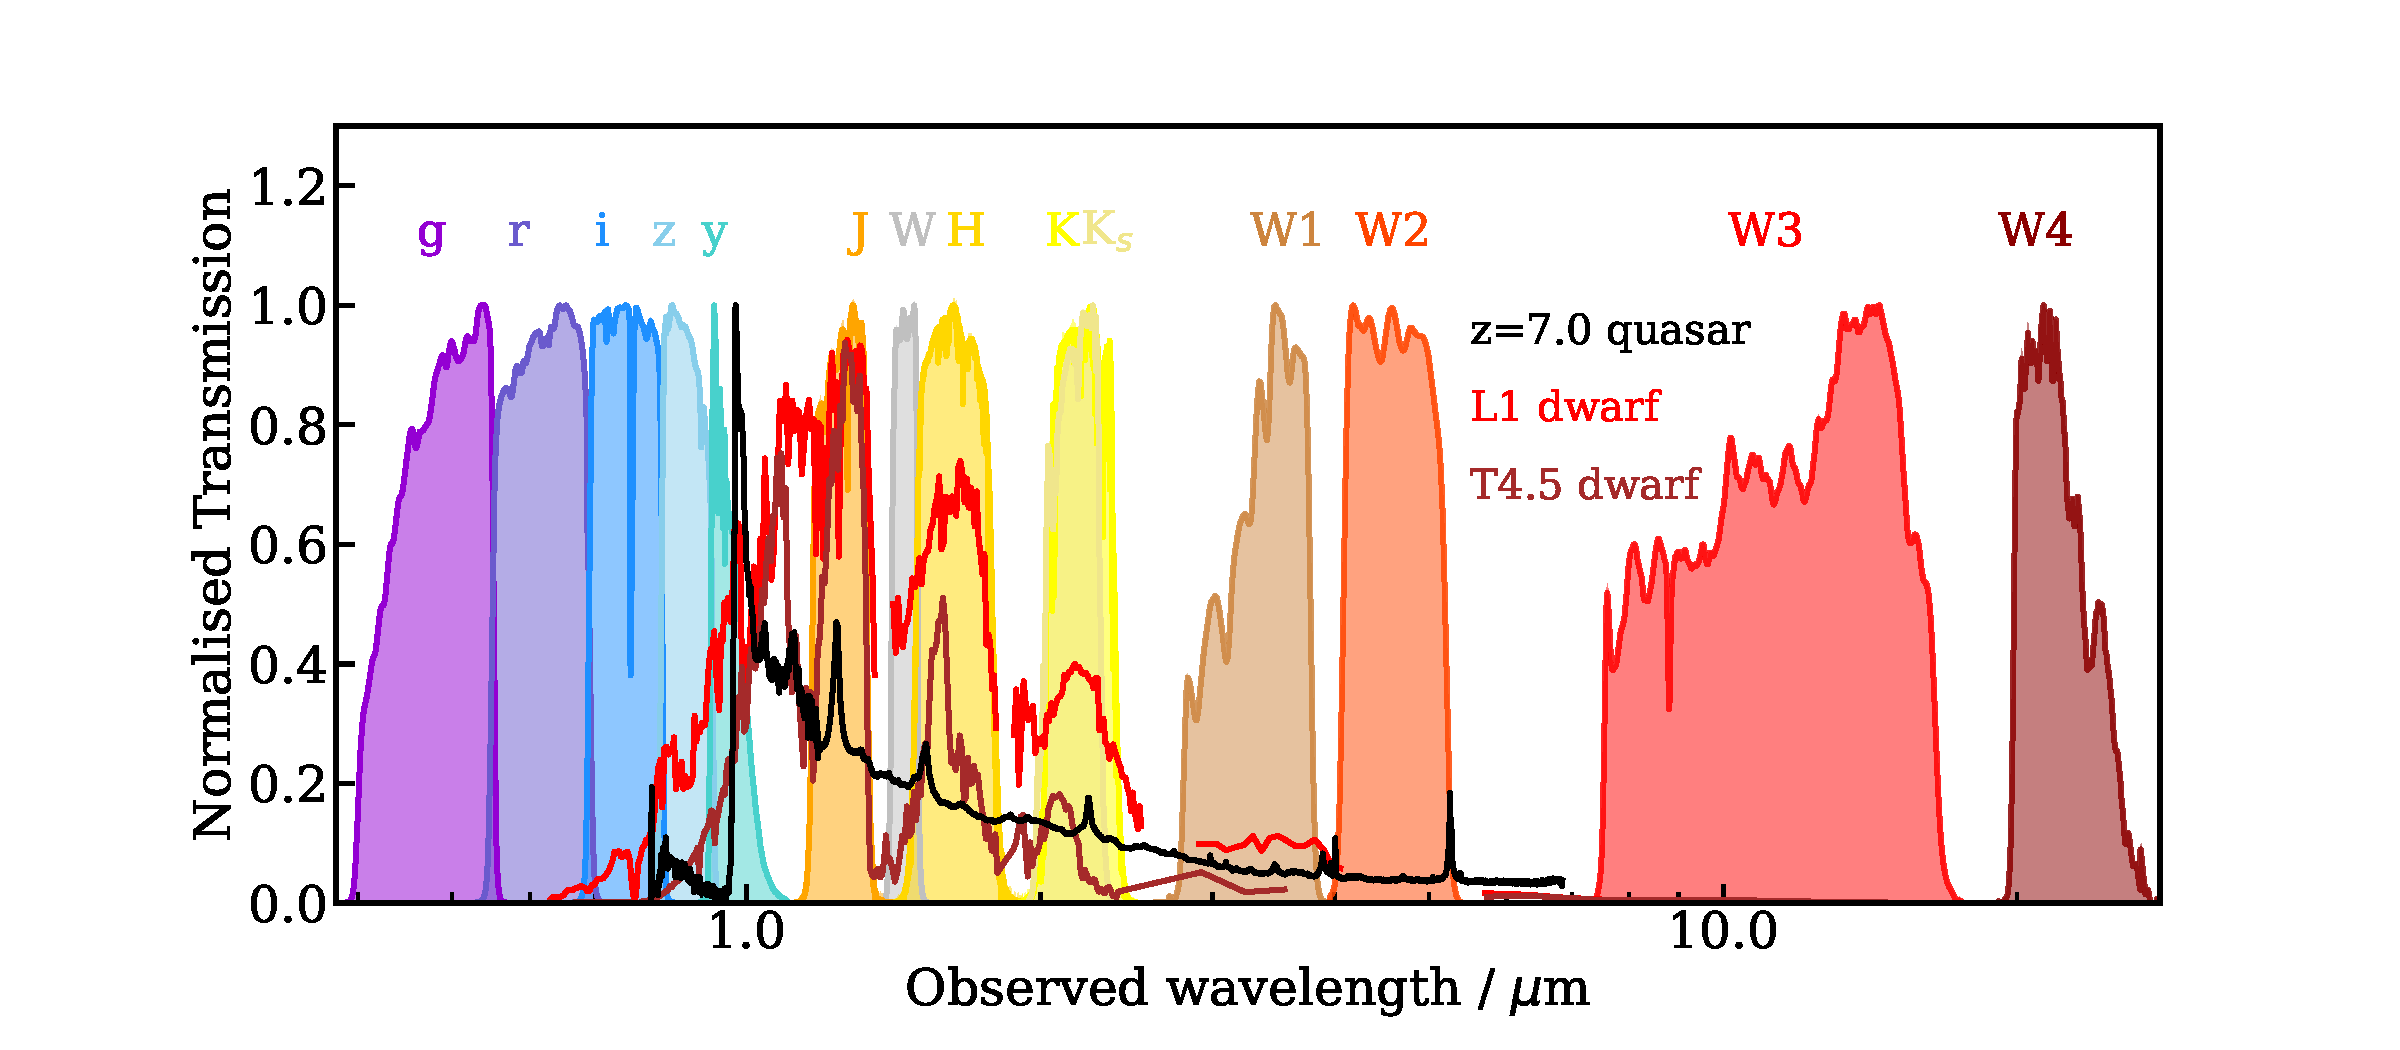
\includegraphics[width=8.6cm, clip,trim=32mm 4mm 32mm 10mm]
  {/cos_pc19a_npr/programs/quasars/highest_z/SEDs/filters_vs_QSOstars_20180704.pdf}
  \centering
  \vspace{-12pt}
  \caption[]
  {The spectral bands used by different survey telescopes and that are relevant here.
    The $grizy$ filters are from the Pan-STARRS survey. The $JHK$ are from 
    UKIRT/WFCAM, while $K_{s}$ is a VISTA/VIRCAM filter. The 
    The narrow W-band centered at $\lambda\approx14,500$\AA\ is a CFHT/Wircam filter. 
    [NJC: Do we use the W-band anywhere?]
    The WISE passbands  W1-4 are also presented.
    The quasar spectrum is a composite based on \citet{VdB2001} and 
    \citet{Banados2016}. The L and T dwarf spectra are from \citet{Cushing2006}. 
  }
  \label{fig:filters}
\end{figure}

\vspace{-16pt}
\section{Data}
In Table~\ref{tab:THE_TABLE} we present our dataset and 
we have assembled this in the following manner.  First
we compile the list of all known, spectroscopically confirmed quasars
from the literature. Most of these objects are easily identified by
their broad Ly$\alpha$ emission line, \nv emission and characteristic
shape blueward of 1215\AA\ observed. As we shall see, some of the more
recently discovered objects are close to the galaxy luminosity
function characteristic luminosity $M^{*}$, and some have relatively
weak or maybe even completely absorbed Ly$\alpha$ \citep[e.g. Figures
7 and 10 in][]{Banados2016}. We leave aside detailed investigation and
discussion into espectral features and line strengths, and take as given 
the published spectra. 

We then obtain optical, near-infrared and mid-infrared photometry for the
spectral dataset. The optical data comes from the 
Panoramic Survey Telescope and Rapid Response System (Pan-STARRS) 
survey \citep{Chambers2016} and the Dark Energy Camera \citep{Flaugher2015}, 
including the Dark Energy Survey \citep[DES;][]{Flaugher2005} and 
the Dark Energy Camera Legacy Survey \citep[DECaLS]{Dey2018}. 

Recently, Hyper Suprime-Cam \citep[HSC; ][]{Miyazaki2018} has embarked
on the Subaru Strategic Program \citep[SSP; ][]{Aihara2018a}
delivering exquisite multi-band photometry data
\citep[][]{Aihara2018b} the five broad bands $grizy$.

The near-infrared data comes from two primary sources. First, the Wide
Field Camera \citep[WFCAM; ][]{Casali2007} on the the United Kingdom
Infra-Red Telescope (UKIRT) primarly, but not exclusively as part of
the UKIRT Infrared Deep Sky Survey \citep[UKIDSS; ][]{Lawrence2007}.
And second, data from the VIRCAM (VISTA InfraRed CAMera) on the VISTA
\citep[Visible and Infrared Survey Telescope for
Astronomy;][]{Emerson2006, Dalton2006}.

We also obtain mid-infrared, $\lambda=3-30\mu$m wavelength data from the
the Wide-Field Infrared Survey Explorer \citep[WISE;][]{Wright2010, Cutri2013} mission.
WISE mapped the sky in 4 passbands, in bands centered at wavelengths of 3.4, 4.6, 12, and 23$\mu$m. 
In total the release all sky ``ALLWISE'' catalog, contains nearly 750 million detections at high-significance\footnote{
\href{http://wise2.ipac.caltech.edu/docs/release/allwise/}{wise2.ipac.caltech.edu/docs/release/allwise/}}. 


Figure~\ref{fig:filters} displays the wavelength and normalised transmission 
of the filters in question. 


%\pagestyle{empty}
\begin{landscape}
%\onecolumn
 % \begin{landscape}
%\small  %\footnotesize \scriptsize \tiny

%%%%%%%%%%%%%%%%%%%%%%%%%%%%%%%%%%%%%%%%%%%%%%%%%%%%%%%%%%%%%%%%%%%%%%%%%%%%%%%%
%%
%%
%%     T A B L E    O N E                GENERAL PROPERTIES,          incl.   redshift   and   M_1450
%%
%%
%%%%%%%%%%%%%%%%%%%%%%%%%%%%%%%%%%%%%%%%%%%%%%%%%%%%%%%%%%%%%%%%%%%%%%%%%%%%%%%%
\begin{table}
\begin{center}
\begin{tabular}
%{|l|l|l|l|r|r|r|r|r|r|r|r|r|r|r|r|r|r|r|r|r|r|r|r|l|}
%{ l l l l r r r r r r r r r r r r r r r r r r r r l }
{ l l   r r  r r   l   l l l   }
\hline \hline
  \multicolumn{1}{ c }{na} &
  \multicolumn{1}{c }{desig} &
  \multicolumn{1}{c }{ra\_hms} &
  \multicolumn{1}{c }{dec\_dms} &
  \multicolumn{1}{c }{ra} &
  \multicolumn{1}{c }{dec} &
  \multicolumn{1}{c }{redshift} &
  \multicolumn{1}{c }{mag} &
  \multicolumn{1}{c }{M1450} &
  \multicolumn{1}{c }{ref} \\
\hline
  PSO & J000.3401+26.8358   & 00:01:21.63 & +26:50:09.17 &   0.340113    &  +26.83588      &   5.75    & 19.52 & -27.16     & 1/1/1\\
  SDSS & J0002+2550             & 00:02:39.39 & +25:50:34.80 &   0.664117    &  +25.84304      &  5.82    & 19.39 & -27.31     & 5/22/1\\
  SDSS & J0005-0006             & 00:05:52.34 & -00:06:55.80 &    1.468083    &  -00.11549      & 5.85    & 20.98 & -25.73     &  5/12/1\\
  PSO & J002.1073-06.4345   & 00:08:25.77 & -06:26:04.60 &    2.107390    &  -06.43456            & 5.93   & 20.41 & -26.32      &   1;43/1/1\\
  SDWISE & J0008+3616         & 00:08:51.43 & +36:16:13.49 &   2.214292    &   +36.27041        & 5.17   & 19.12 & -27.34     &    Wang2016\\
  PSO & J002.3786+32.8702  & 00:09:30.89 & +32:52:12.94 &    2.378702   &   +32.87026     &  6.1     & 21.13  & -25.65    &  1/1/1\\
  SDSS & J0017-1000             & 00:17:14.68 & -10:00:55.4 &      4.311166   &    -10.01540    & 5.011  & 99.99 & -99.99     &   DR7\_W16\\
  PSO & J004.3936+17.0862  & 00:17:34.47 & +17:05:10.70 &    4.393614   &   +17.08631      & 5.8      & 20.69 & -26.01     &  1/1/1\\
  PSO & J004.8140-24.2991  & 00:19:15.38 & -24:17:56.98 &     4.814080   &   -24.29920          & 5.68      & 19.43 & -27.24      &    1/1/1\\
  VDES & J0020-3653            & 00:20:31.46 & -36:53:41.8 &       5.131124   &   -36.89495       & 6.9      & 99.99 & -99.99       &   DES-VHS\_inprep\\
\hline \hline
\end{tabular}
\caption{All 424 $z\geq5.00$ quasars that have been spectroscopically confirmed as of 2018 June. 
  The first ten objects are given here as guidance to the format of the data table. The full table  can be found online.} 
\label{tab:THE_TABLE}
  \end{center}
\end{table}
\normalsize 

%  \end{landscape}
%\twocolumn
%\pagestyle{plain}


\medskip
\medskip

%\pagestyle{empty}
%\begin{landscape}
%\onecolumn
 % \begin{landscape}
%\small  %\footnotesize \scriptsize \tiny

%%%%%%%%%%%%%%%%%%%%%%%%%%%%%%%%%%%%%%%%%%%%%%%%%%%%%%%%%%%%%%%%%%%%%%%%%%%%%%%%
%%
%%
%%     T A B L E     T W O                     NEAR     IR     PROPERTIES         
%%
%%
%%%%%%%%%%%%%%%%%%%%%%%%%%%%%%%%%%%%%%%%%%%%%%%%%%%%%%%%%%%%%%%%%%%%%%%%%%%%%%%%
\begin{table}
\begin{center}
\begin{tabular}
%{|l|l|l|l|r|r|r|r|r|r|r|r|r|r|r|r|r|r|r|r|r|r|r|r|l|}
%{ l l l l r r r r r r r r r r r r r r r r r r r r l }
{ l l l l l l l l l l l l l l l l l l l l l l l l l }
\hline \hline
  \multicolumn{1}{ c }{na} &
  \multicolumn{1}{c }{desig} &
  \multicolumn{1}{c }{ra} &
  \multicolumn{1}{c }{dec} &
  \multicolumn{1}{c }{w1mag} &
  \multicolumn{1}{c }{w1err} &
  \multicolumn{1}{c }{w1snr} &
  \multicolumn{1}{c }{w2mag} &
  \multicolumn{1}{c }{w2err} &
  \multicolumn{1}{c }{w2snr} &
  \multicolumn{1}{c }{w3mag} &
  \multicolumn{1}{c }{w3err} &
  \multicolumn{1}{c }{w3snr} &
  \multicolumn{1}{c }{w4mag} &
  \multicolumn{1}{c }{w4err} &
  \multicolumn{1}{c }{w4snr} \\
\hline
  PSO & J000.3401+26.8358   &   0.34011348  & 26.83588138     & 16.373      & 0.066  & 16.5 &    15.266 & 0.107 & 10.2 & 12.594 & 0.492 & 2.2 & 8.756 & -9.99 & 1.1 \\
  SDSS & J0002+2550             &   0.66411726  & 25.84304425     & 16.162      & 0.057  & 19.0 &    15.542 & 0.127 & 8.5 & 12.416 & 0.423 & 2.6 & 8.683 & -9.99 & 1.2 \\
  SDSS & J0005-0006             &    1.4680833   & -0.1154999        & 17.299      & 0.16   &  6.8 &      17.043 & -9.99 & 0.2 & 12.445 & -9.99 & -1.1 & 9.008 & -9.99 & -0.3 \\
  PSO & J002.1073-06.4345   &    2.10739       & -6.43456            &  16.809     & 0.107 & 10.1 &     15.684 & 0.141 & 7.7 & 11.892 & -9.99 & 1.5 & 8.759 & -9.99 & 0.2  \\
  SDWISE & J0008+3616         &    2.2142917   & 36.2704138        &  16.045     & 0.052 & 20.7 &     15.373 & 0.092 & 11.8 & 12.043 & -9.99 & 1.8 & 8.786 & -9.99 & 1.1 \\
  PSO & J002.3786+32.8702   &   2.37870183  & 32.87026179      &  -99.99     & -9.99  & -9.9 &   -99.99 & -9.99 & -9.9 & -99.99 & -9.99 & -9.9 & -9.99 & -9.99 & -9.9 \\
  SDSS & J0017-1000              &   4.3111666   & -10.01539722     & 15.936      & 0.055 & 19.7 &     15.167 & 0.094 & 11.5 & 12.026 & 0.334 & 3.2 & 8.52 & -9.99 & 1.2 \\
  PSO & J004.3936+17.0862   &   4.39361347  & 17.08630447      &  -99.99     & -9.99  & -9.9 &    -99.99 & -9.99 & -9.9 & -99.99 & -9.99 & -9.9 & -9.99 & -9.99 & -9.9 \\
  PSO & J004.8140-24.2991   &   4.81408        & -24.29916           &  16.281    & 0.069 & 15.8 &      15.569 & 0.116 & 9.4 & 12.123 & 0.344 & 3.2 & 8.82 & -9.99 & 0.5 \\
  VDES & J0020-3653             &   5.1311237     & -36.8949476      &  16.844  & 0.094 & 11.6 &        16.354 & 0.204 & 5.3 & 12.679 & -9.99 & -0.1 & 8.342 & -9.99 & 0.8 \\
\hline \hline
\end{tabular}
\caption{The mid-infrared photometric properties from the WISE ALLWISE
catalogue for the 424 very-high redshift quasars.  The first ten
objects are given here as guidance to the format of the data
table. The full table can be found online.  {\it This is the third
table here; the SECOND table is this with the NIR data...}}
\label{tab:THE_TABLE_NIR}
  \end{center}
\end{table}
\normalsize 

%  \end{landscape}
%\twocolumn
%\pagestyle{plain}


\medskip
\medskip


%\pagestyle{empty}
%\begin{landscape}
%\onecolumn
 % \begin{landscape}
%\small  %\footnotesize \scriptsize \tiny
%%%%%%%%%%%%%%%%%%%%%%%%%%%%%%%%%%%%%%%%%%%%%%%%%%%%%%%%%%%%%%%%%%%%%%%%%%%%%%%%
%%
%%
%%     T A B L E     T H R E E                     MID    IR     PROPERTIES           from     WISE ALLWISE
%%
%%
%%%%%%%%%%%%%%%%%%%%%%%%%%%%%%%%%%%%%%%%%%%%%%%%%%%%%%%%%%%%%%%%%%%%%%%%%%%%%%%%
\begin{table}
\begin{center}
\begin{tabular}
%{|l|l|l|l|r|r|r|r|r|r|r|r|r|r|r|r|r|r|r|r|r|r|r|r|l|}
%{ l l l l r r r r r r r r r r r r r r r r r r r r l }
{ l l l l l l l l l l l l l l l l l l l l l l l l l }
\hline \hline
  \multicolumn{1}{ c }{na} &
  \multicolumn{1}{c }{desig} &
  \multicolumn{1}{c }{ra} &
  \multicolumn{1}{c }{dec} &
  \multicolumn{1}{c }{w1mag} &
  \multicolumn{1}{c }{w1err} &
  \multicolumn{1}{c }{w1snr} &
  \multicolumn{1}{c }{w2mag} &
  \multicolumn{1}{c }{w2err} &
  \multicolumn{1}{c }{w2snr} &
  \multicolumn{1}{c }{w3mag} &
  \multicolumn{1}{c }{w3err} &
  \multicolumn{1}{c }{w3snr} &
  \multicolumn{1}{c }{w4mag} &
  \multicolumn{1}{c }{w4err} &
  \multicolumn{1}{c }{w4snr} \\
\hline
  PSO & J000.3401+26.8358   &   0.34011348  & 26.83588138     & 16.373      & 0.066  & 16.5 &    15.266 & 0.107 & 10.2 & 12.594 & 0.492 & 2.2 & 8.756 & -9.99 & 1.1 \\
  SDSS & J0002+2550             &   0.66411726  & 25.84304425     & 16.162      & 0.057  & 19.0 &    15.542 & 0.127 & 8.5 & 12.416 & 0.423 & 2.6 & 8.683 & -9.99 & 1.2 \\
  SDSS & J0005-0006             &    1.4680833   & -0.1154999        & 17.299      & 0.16   &  6.8 &      17.043 & -9.99 & 0.2 & 12.445 & -9.99 & -1.1 & 9.008 & -9.99 & -0.3 \\
  PSO & J002.1073-06.4345   &    2.10739       & -6.43456            &  16.809     & 0.107 & 10.1 &     15.684 & 0.141 & 7.7 & 11.892 & -9.99 & 1.5 & 8.759 & -9.99 & 0.2  \\
  SDWISE & J0008+3616         &    2.2142917   & 36.2704138        &  16.045     & 0.052 & 20.7 &     15.373 & 0.092 & 11.8 & 12.043 & -9.99 & 1.8 & 8.786 & -9.99 & 1.1 \\
  PSO & J002.3786+32.8702   &   2.37870183  & 32.87026179      &  -99.99     & -9.99  & -9.9 &   -99.99 & -9.99 & -9.9 & -99.99 & -9.99 & -9.9 & -9.99 & -9.99 & -9.9 \\
  SDSS & J0017-1000              &   4.3111666   & -10.01539722     & 15.936      & 0.055 & 19.7 &     15.167 & 0.094 & 11.5 & 12.026 & 0.334 & 3.2 & 8.52 & -9.99 & 1.2 \\
  PSO & J004.3936+17.0862   &   4.39361347  & 17.08630447      &  -99.99     & -9.99  & -9.9 &    -99.99 & -9.99 & -9.9 & -99.99 & -9.99 & -9.9 & -9.99 & -9.99 & -9.9 \\
  PSO & J004.8140-24.2991   &   4.81408        & -24.29916           &  16.281    & 0.069 & 15.8 &      15.569 & 0.116 & 9.4 & 12.123 & 0.344 & 3.2 & 8.82 & -9.99 & 0.5 \\
  VDES & J0020-3653             &   5.1311237     & -36.8949476      &  16.844  & 0.094 & 11.6 &        16.354 & 0.204 & 5.3 & 12.679 & -9.99 & -0.1 & 8.342 & -9.99 & 0.8 \\
\hline \hline
\end{tabular}
\caption{The mid-infrared photometric properties from the WISE ALLWISE
catalogue for the 424 very-high redshift quasars.  The first ten
objects are given here as guidance to the format of the data
table. The full table can be found online.  {\it This is the third
table here; the SECOND table is this with the NIR data...}}
\label{tab:THE_TABLE_MIR}
  \end{center}
\end{table}
\normalsize 
  \end{landscape}
\twocolumn
%\pagestyle{plain}



\subsection{Spectroscopy} 
We have obtained a list of 424 spectroscopically confirmed 
quasars with redshifts $z\geq5.00$. 

In Table~\ref{tab:THE_TABLE}  we give the discovery reference for the
VH$z$Qs noting that some objects were discovered independently and
contemporaneously.  The redshifts for the VH$z$Qs generally come from
the measurement of broad UV/optical emission lines. Where 
there are far infra-red emission lines e.g. \cii~158 micron, we report 
these, but at the level of our current analysis broadline redshifts are
sufficient. 

Specifically, we use data from: \citet{Fan2000}, \citet{Fan2001c},
\citet{Fan2003}, \citet{Fan2004}, \citet{Mahabal2005},
\citet{Cool2006}, \citet{Fan2006}, \citet{Goto2006},
\citet{McGreer2006}, \citet{Carilli2007}, \citet{Kurk2007},
\citet{Stern2007}, \citet{Venemans2007}, \citet{Willott2007},
\citet{Jiang2008}, \citet{Wang2008}, \citet{Jiang2009}, \citet{Kurk2009}, 
\citet{Mortlock2009}, \citet{Willott2009}, \citet{Carilli2010}, 
\citet{Wang2010}, \citet{Willott2010a}, \citet{Willott2010b}, 
\citet{DeRosa2011}, \citet{Mortlock2011}, \citet{Wang2011}, 
\citet{Zeimann2011}, \citet{Morganson2012}, \citet{Venemans2012}, 
\citet{McGreer2013}, \citet{Venemans2013}, \citet{Wang2013}, 
\citet{Willott2013b}, \citet{Banados2014}, \citet{Calura2014}, 
\citet{Leipski2014}, \citet{Banados2015a}, \citet{Banados2015b}, 
\citet{Becker2015}, \citet{Carnall2015}, \citet{Jiang2015}, 
\citet{Kashikawa2015}, \citet{Kim2015}, \citet{Reed2015}, 
\citet{Venemans2015a}, \citet{Venemans2015b}, \citet{Willott2015}, 
\citet{Wu2015}, \citet{Venemans2016}, \citet{Wang2016_WISE}, 
\citet{Matsuoka2016}, \citet{WangR2016}, \citet{Mortlock2011},
\citet{McGreer2013}, \citet{Venemans2013}, \citet{Venemans2013},
\citet{Venemans2015a}, \citet{Venemans2015b}, \citet{Banados2016},
\citet{Matsuoka2016}, \citet{Reed2017}, \citet{Wang2017},
\citet{Mazzucchelli2017}, \citet{Ikeda2017}, \citet{Tang2017},
\citet{Koptelova2017}, \citet{Banados2018}, \citet{Matsuoka2018a} 
and \citet{Matsuoka2018b}. 

Table~\ref{tab:THE_TABLE} gives the salient details for the objects
used in this study. We use all the $z\geq5.00$ quasars that
have been discovered and spectroscopically confirmed as of the time of
writing (2018 June). We report near-infrared ($yYJHK$-bands)
and mid-infrared (WISE W1/2/3/4) photometry and give our caculcated 
$M_{1450}$. 

\begin{table}
\begin{tabular}{l r l}
\hline  \hline
Survey   & \# VH$z$Qs & Notes/Survey reference  \\
\hline  
  ATLAS      &     4    &  \citet{Shanks2015} \\
  CFHQS     &   20    &  \citet{Willott2007} \\
  DELS        &     2    &  \citet{Dey2018} \\
  ELAIS       &     1    &  \citet{Vaisanen2000} \\
  FIRST       &     1    &  \citet{Becker1995} \\
%  HSC         &     8    &  \\
  IMS          &     1     &  \citet{Kim2015} \\
  MMT        &   12    &  \citet{McGreer2013} \\
  NDWFS    &     1     &  \citet{JD1999} \\
  PSO          &   84    &   \citet{Kaiser2002, Kaiser2010} \\
  RD           &     1       &  \cite{Mahabal2005} \\
  SDSS        & 156       & \citet{EDR} \\
  SDUV       &   20       & \citet{Yang2017} \\
  SDWISE    &   27    &     \citet{Wang2016} \\
  SHELLQs  &  $^{a}$63   &  \citet{Matsuoka2016}\\  %% includes 8 objects from the first HSC paper..
  ULAS       &   10   & \citet{Lawrence2007} \\
  VDES       &   11   &  \citet{Reed2017} \\
  VIK          &     9   &  \citet{Edge2013} \\
  VIMOS     &     1   &  \citet{LeFevre2003} \\
\hline  \hline
\end{tabular}
\caption{The number of VH$z$Q from given surveys, with the key survey or telescope reference. 
$^{a}$Includes 8 objects with a HyperSuprimeCam \citep[HSC; ][]{Miyazaki2018}  
designation.
}
      \label{tab:surveys}
\end{table}

        
\subsection{Optical Photometry}
    \subsubsection{Pan-STARRS1 (PS1)} 
    We query the Panoramic Survey Telescope and Rapid Response System
    (Pan-STARRS)\footnote{\href{https://outerspace.stsci.edu/display/PANSTARRS}{https://outerspace.stsci.edu/display/PANSTARRS}}
    Data Release 1 (DR1) Catalog Archive Server Jobs System (CasJobs)
    service at
    \href{http://mastweb.stsci.edu/ps1casjobs/}{mastweb.stsci.edu/ps1casjobs/}.
    The PS1 survey observed the 30,000 deg$^{2}$ of sky north of
    declination $-30$ degrees in five filters $grizy$.  Pan-STARRS1 (PS1)
    is the first part of Pan-STARRS to be completed and is the basis for
    the DR1.  \citet{Chambers2016}, \citet{Magnier2016a},
    \citet{Waters2016}, \citet{Magnier2016b}, \citet{Magnier2016c} and
    \citet{Flewelling2016} describe the instrument, survey, and data
    analyses.  The principal science product of the PS1 survey is the
    catalog accessible through the CasJobs interface.
    
    We query and return the mean PSF magnitudes from the $grizy$ filters
    ({\tt MeanPSFMag}) which are in the AB system for our 424 VH$z$Q
    sample. Details of our SQL and links to the main tables are given
    in Appendix~\ref{sec:PS1_SQL}.
    
    \iffalse
    \subsubsection{DECam} 
    The Dark Energy Camera \citep[DECam][]{Flaugher2015} is 
    is a wide-field imager with a 2.2 degree diameter field of view 
    mounted at the prime focus of the Victor M. Blanco 4 m telescope 
    at the Cerro Tololo International Observatory. We use data 
    from both the Dark Energy Survey \citep[DES; ][]{DES2016} and 
    the DESI Legacy Imaging Survey \citep[DECaLS; ][]{Dey2018}. 
    \fi
    

\subsection{Near-infrared photometry}~\label{sec:NIR_data} 
Due to their selection of being very faint/undetected in the
observed-frame optical but bright in the observed frame near-infrared,
VH$z$Qs are generally detected in the near-infrared $yYJHK$-bands
\citep[$\approx$0.98-2.38$\mu$m; e.g., ][]{Peth2011}.

The near-infrared data in this paper comes from the Wide Field Astronomy Unit's
(WFAU) Science Archives for UKIRT-WFCAM, the WFCAM Science Archive
\citep[WSA][]{WSA} and VISTA-VIRCAM, the VISTA Science Archive
\citep[VSA][]{VSA}. These archives were developed for the VISTA Data Flow System
\citep[VDFS][]{VDFS}.

In this paper we include all non-proprietary WFCAM data, which covers all
public surveys and PI projects from Semester 05A to 1st January 2017 and all
non-proprietary VISTA data, which covers all public surveys and PI projects from
science verification (20091015) to 1st April 2016, to get as much coverage as
possible. Hence, the NIR coverage is extremely heterogeneous. 

The data was processed using a forced photometry, or matched-aperture
photometry. A pipeline for this has been developed by WFAU, but
has not yet been incorporated into the main VDFS pipeline. Full details of the
matched-aperture pipeline (MAP) will appear in a forthcoming paper, Cross et al.
2018, in prep, and has also been discussed in \citet{Cross2013}.  
%% and \citet{Cross2017} -- Can't find Cross et al. 2017 in NASA/ADS. [NJC: this was a conference proceeding
%% from ADASS2016. They just contacted me about the copyright. They are so slow even though we 
%% had to submit our proceedings before the conference. I had assumed it was already published.]
We will give the pertinent points of the MAP and specific details of these data sets below.
   
The first step of the process was to ingest the catalogue of VHzQs into
the WSA/VSA. These data are stored in the table \verb+finalQsoCatalogue+. Next we set
up new programmes WSERV1000, VSERV1000 in the WSA and VSA respectively. We
assign all frames that potentially contain the high-z QSO based on WCS information in the
WSA to WSERV1000, but adding a new line to the table \verb+ProgrammeFrame+ and
same in VSA for VSERV1000. Assigning these frames to a separate programme allows
us to process them together and put them into a single release. 
    
\subsubsection{Setup Matched Aperture Product}
To create matched aperture products it is first necessary to define
the product. We do this in two requirements tables,
\verb+RequiredMatchedApertureProduct+ and \verb+RequiredMapAverages+
that tell the \textbf{ProgrammeBuilder} software which tables to
create and what type of product is being created. These requirements
tables also drive the pipeline.

\verb+RequiredMatchedApertureProduct+ contains the following attributes for the High-z QSO MAP product.
\begin{itemize}
    \item mapID, Identifier of the MAP product, value=1	
    \item archiveName, Main archive of product, value='VSA'/'WSA' 	
    \item programmeID, UID of programme, in this case a combined programme, value=10999
    \item extractor, Extractor used for forced photometry, value='CASU' (imcore\_list)
    \item mapType, Type of MAP product (options 0 internal band-merged, 1 band-merged across surveys, 2 multi-epoch), value=2 
    \item name, Name of MAP product, value='highzQsoMap'
    \item description, Description of MAP product, 'Variability via matched apertures for set of high-z QSOs'	
    \item selection, Selection, e.g. File, pseudo-SQL, FITS image that is used to give input list, value='SELECTSTR qsoID,ra,dec FROMSTR finalQsoCatalogue'	
    \item finalProductTable, Name of final product table, value='highzQsoMapVariability'
    \item addSurveyList, List of additional archive/surveys that data comes from, value='NONE'
\end{itemize}
    
\verb+RequiredMatchedApertureProduct+ gives all of the information such as the {\it programmeID} (identifying which data), the {\it mapType} (type of processing), the {\it extractor} to use, the input list {\it selection}, which in this case is the IDs and positions of the QSOs in \verb+finalQsoCatalogue+ which contains all the literature data and pre-derived parameters for the 424 QSOs.   
    
\verb+RequiredMapAverages+ is used to setup the averaging of the MAP photometry from several images. We can average the epochs in multiple ways: over all the input images to a deep image, or similarly the input pawprint images to tile image in VISTA. Alternatively we can average over a fixed number of epochs or a fixed duration in time. Multiple setups can be defined in \verb+RequiredMapAverages+, and the different averages selected using the defined {\it setupID}.
    
    Add table?
    \begin{table*}
      \begin{center}
        \setlength{\tabcolsep}{4pt}
        \begin{tabular}{ll lll lll l}
          \hline \hline
   programmeID &	mapID &	setupID  &	description               &	useDeeps  &	useHighProd &	timeScale	    &  nEpochs     &	overLaps\\
          \hline
10999	& 1 & 0 & Average over whole time & 0 &	NONE &	-1.000000 &	-99999999 &	1 \\
10999	& 1 & 1 & Average over a week &	0 & NONE & +7.000000 &	-99999999 &	1\\
10999	& 1 & 2	& Average over a fortnight & 0 & NONE &	+14.000000 & -99999999 & 1\\
10999	& 1 & 3	& Average over a month & 0 & NONE & +30.000000 & -99999999 & 1\\
10999	& 1 & 4	& Average over 10 epochs & 0 & NONE & -9.999995E008 & 10 & 1\\
10999	& 1 & 5 & Average over 6 months	& 0 & NONE & +183.000000 & -99999999 & 1 \\
10999	& 1 & 6	& Average over 1 year &	0 & NONE & +365.000000 & -99999999 & 1 \\
10999	& 1 & 7	& Average over 2 years & 0 & NONE & +730.000000	& -99999999 & 1 \\
10999	& 1 & 8 & Average over 3 months & 0 & NONE & +91.000000	& -99999999 & 1 \\
          \hline \hline
          \label{tab:reqMapAvg}
        \end{tabular}
        \caption{}
      \end{center}
    \end{table*}
    
    
    \subsubsection{Processing MAP data and Forced photometry} 
    A set of apertures to do forced photometry with were created in 
    \verb+MapApertureIDshighzQsoMap+, based on the \verb+RequiredMatchedApertureProduct+ 
    {\it selection} value, which in this case is to use the known positions of $z>5$ QSOs. This may
    seem unnecessary layer since it is a one-to-one match with \verb+finalQsoCatalogue+,
    but the layer is a general abstraction that allows multiple selections of data, including complex queries
    or input images.
    
    CASU's \verb+imcore_list+ was run on each frame assigned to the programme with
    the input list equal to objects selected to be within \ldots of the multiframe
    centre. In this case, where there are 424 QSOs spread across the sky, there is
    typically 1 object per multiframe, but many have two and one frame,
    multiframeID=2614475 in the VSA (a J-band stack from a P90 PI programme), has 3 objects. 
    The output of \verb+imcore_list+
    is a multi-extension FITS binary table, with identical columns to the CASU FITS
    binary tables produced using the CASU \verb+imcore+\footnote{http://casu.ast.cam.ac.uk/surveys-projects/vista/technical/catalogue-generation}, the basis of all WFCAM and
    VISTA survey catalogue products and also familiar to many astronomers through the INTWFS, 
    VST-ATLAS and VPHAS. Since forced photometry can be run
    in many ways on a particular image depending on the input catalogue, a single science frame is not
    necessarily linked to a single MAP catalogue, so the \verb+MapFrameStatus+ table
    links images ({\bf multiframeID}) to catalogues ({\bf catalogueID}).
    For matched aperture measurements, we process these binary tables using the same
    software, as the standard extracted catalogues, but implement a few different
    processes. We calculate both Luptitudes \citep{Luptitudes}, and calibrated fluxes,
    see Eqn~\ref{eq:jky}. 
    
    \begin{equation}
      F^{calib} = f\times10^{-0.4*(ZP+VAB-8.90+corr)} 
      \label{eq:jky}
    \end{equation}
    
    \noindent where $f$ is the measured flux in ADU, $ZP$ is the zeropoint of
    frame, $VAB$ is the Vega-to-AB correction for the filter, and $corr$ are the
    various correction terms, e.g. distortion correction, scattered light
    correction, aperture correction, see \citep{Hambly2008, Cross2012}. 
    
    Once all data is processed, the data are ingested into
    \verb+wserv1000MapRemeasurement+ and \verb+vserv1000MapRemeasurement+
    respectively. These tables are similar in structure to \verb+lasDetection+
    described in \citep{Hambly2008} or other UKIDSS or VISTA detection tables. One of
    the main differences is the primary key which is ({\bf apertureID},{\bf
      catalogueID}) rather than ({\bf multiframeID},{\bf extNum},{\bf seqNum}),
    reflecting the fact that these are forced photometry on a known set of apertures
    and a set of catalogues, rather than detections above a threshold in a set of
    detector extensions to image multiframes.
    
    Quasars are known to vary (both photometrically and spectroscopically)
and very high-$z$ quasars under going super-Eddington accretion during
a rapid BH growth phase are prime candidates for this variation. [NJC: This is better placed somewhere else. We first used it to justify averaging over ~4 weeks, but then decided to average over many periods and select later.]
Therefore, with repeat observations over many epochs available via the
WSA, we have a choice to make for how we report the photometry. The remeasured photometry is averaged to
improve signal-to-noise over all the averaging schemes setup in Table~\ref{tab:reqMapAvg}. This allows us to get the best combination of signal-to-noise and number of epochs for different QSOs.

    
    \subsubsection{Averaging matched photometry}
    Unfortunately the photometry in a single epoch image often has low
    signal-to-noise. The advantage of matched aperture photometry on QSOs is that
    co-adding is relatively simple: if each epoch is taken in the same aperture
    (assuming the astrometry is correct) and the aperture photometry has been
    corrected to total: the standard aperture corrections work well for point
    sources then averaging the calibrated photometry should give as good as
    extracting from a deep stack. In fact it will almost certainly do better, since
    the images in some cases are taken from multiple projects with different
    pointings, and orientations and exposures, so stacking may not be optimal. 
    In addition, corrections such as scattered light, pixel distortion
    and aperture corrections will be more complex, if not impossible to apply to
    deep-stacks but will be automatically applied in the averaging of forced
    photometry. 
    
    We average the aperture corrected calibrated fluxes (e.g. {\bf aperJky3}), and
    then convert to magnitudes or luptitudes. Since we do not have a deep image for
    each set of averages, we cannot calculate non-aperture corrected values, so the
    photometry is only appropriate for point-sources. 
    
    \begin{equation}
      \bar{F} = \frac{\sum_i^N (w_i\,F_i)}{\sum_i^N w_i}  
      \label{eq:avg}
    \end{equation}
    
    \noindent where $F_i$ is the $i^{th}$ epoch measurement of a parameter to be
    averaged such as the aperture corrected calibrated flux in a $1\arcsec$ aperture
    ({\bf aperJky3}) and $\bar{F}$ is the weighted mean average of this parameter.
    The weight for each epoch $w_i=1/(\sigma_{F})^2$ if the epoch is included and 
    $w_i=0$ if an epoch is excluded for quality control purposes. We exclude inputs
    where the bitwise quality flag, {\bf ppErrBits}>256, and additionally, in the
    case of VISTA, we exclude data on detector 16 ({\bf extNum=17}), where the 
    quantum efficiency is variable. If all remeasurements are excluded, then one  of
    the ones with the lowest {\bf ppErrBits} is used. In this case the averages 
    will be equal to the original measurement, and the reader may wonder why we 
    bother to duplicate the data. It is important to do this to simplify queries 
    for users who will then not have to set up complex queries to work out where 
    the data is, and only around $2\%$ of VISTA MAP measurements were excluded  so
    the fraction of duplications is very low. The average data is stored in 
    \verb+wserv1000MapRemeasAver+ for WFCAM and \verb+vserv1000MapRemeasAver+ for 
    VISTA, which again are organised with a primary key of ({\bf apertureID},{\bf catalogueID}).
    Some parameters that are averaged do not have an error $\sigma_{F}$, so in these
    cases we weight them using the {\bf averageConf} parameter, which has a median
    of 100. In the case of WFCAM where this is not calculated, we set each epoch to
    have an {\bf averageConf}$=100$. The {\bf sumWeights} parameter in the
    \verb+MapRemeasAver+ tables is the sum of all the {\bf averageConf} values that
    went into the calculation and the \verb+vserv1000MapAverageWeights+ table gives
    the weights for each epoch, linked to each average for VSERV1000. 
    
    We calculate a set of averaged catalogues, for each pointing and filter, based
    on the requirements in \verb+RequiredMapAverages+, in these cases over time
    spans of 7, 14, 30, 91, 183 days, 365 days, 730 days, over 10 epochs and over all epochs,
    see Tab.~\ref{tab:reqMapAvg}. The
    averaging process starts at the first epoch and works on. Possible future
    refinements could first look for denser groupings that satisfied the criteria so
    that these were not split into two groups. For this high-z QSO project we have averaged over overlaps, 
    because in several cases data for one source comes from multiple original projects that have slightly 
    different pointings. 
    
    Each averaged catalogue has a separate entry in
    \verb+MapFrameStatus+ and is linked to each original epoch remeasured catalogue
    through \verb+MapProvenance+, which contains the averaged catalogue
    identifier {\bf combiCatID}, the epoch catalogue identifier {\bf catalogueID}
    and the averaging setup ID {\bf avSetupID}. 

We give our recipe and SQL query syntax in Appendix~\ref{sec:SQL}.



    The code to calculate variability statistics as described in \cite{Cross2009} has
    not yet been completed to run with the matched aperture pipeline, so these are
    not included. Variables were selected ...
    
    
    

\subsubsection{Selection of NIR variables}
To select potentially variable QSOs we first did a selection like
Appendix D(??), selecting the photometry averaged over the whole time
span to assess the overall signal-to-noise, total timespan and number
of measurements. For each QSO in each filter measured by each
instrument, our initial selection for potential variables was $N_{\rm
meas}\geq8$, $T_{\rm tot}=\max{mjd}-\min{mjd}>30.$ days, $F>0.$ Jky
and SNR>8, to give a signal-to-noise of $\sim\geq3$ per epoch and at
least five measurements. An estimate was made of the number of useful
epochs, such that $N_{\rm epc}=\min(N_{\rm
meas},\frac{SNR}{sqrt{3.}}$. This in turn was used to estimate a
typical time-scale for averaging, $T_{\rm avg}=\frac{T_{\rm
tot}}{N_{\rm meas}}$.

We select average photometry where $(T_{\rm
avg}/2.)\leq\verb+RequiredMapAverages.timeScale+\leq(2.*T_{\rm avg})$,
a setup that should give the best combination of more epochs to
resolve the variation and signal-to-noise per epoch. For each setup
which satisfies this criteria, we get the averaged photometry and
check the statistics. We calculate the median, and the
median-absolute-deviation (MAD), and calculate the ratio of the
standard deviation to the typical error, 
$r=\frac{1.48MAD} {{\overline{error}/\sqrt(N_{\rm epochs})}}$. Likely variables have
$rat\geq3.$ and $N_{\rm epoch}\geq4$. Using this selection, we found
two potential variables, xx and yy, both of which show variability in
VISTA, with timescales of xn and ym, respectively. [Put in results]

As stated before, 114 QSOs have both WFCAM and VISTA data, and so some
variables with fewer measurements in each, may also be variables. We
took all of the intially selected variables that had both WFCAM and
VISTA data, and looked for potential timescales in either WFCAM or
VISTA, and if there was at least one good timescale, appropriate
timescales were applied to both WFCAM and VISTA photometry: i.e. if a
timescale of 30 days was found for WFCAM and 90 days for VISTA then
the combined light curve would be averaged over 30 days for WFCAM and
90 days for VISTA; if only a 90 day average timescale for VISTA was
found, then both WFCAM and VISTA would be averaged by 90 days, and if
multiple averaging timescales were found, all suitable combinations
would be tested. The same analysis of median and MAD was applied to
the combined light-curves to find any additional potential
variables. 2 more potential variables were found.



\subsection{MIR data}
The MIR data for this study comes exclusively from the Wide-field
Infrared Survey Explorer (WISE) mission. Since we are only concerned
here with the very large area ($\gg1000$ deg$^2$) surveys, we leave
exploration of the VH$z$Q population in e.g. the large Spitzer areal
surveys such as the Spitzer IRAC Equatorial Survey \citep[SpIES;
][]{Timlin2016}, the Spitzer-HETDEX Exploratory Large-area Survey
\citep[SHELA; ][]{Papovich2016} and the Spitzer-SPT Deep Field
\citep[SSDF; ][]{Ashby2013}, to a future investigation. This will also
include a detailed study of MIR spectra e.g. \citet{Lambrides2018}.

We use data from the the beginning of the WISE mission \citep[2010
January; ][]{Wright2010} through the fourth-year of NEOWISE-R
operations \citep[2017 December;]{Mainzer2011}. More specifically, we
use the data from the
\href{http://wise2.ipac.caltech.edu/docs/release/allwise/}{AllWISE}
program and catalogue, which combines data from the WISE cryogenic and
NEOWISE (Mainzer et al. 2011 ApJ, 731, 53) post-cryogenic survey
phases. For the our variability investigations, we supplement the
ALLWISE data with data from the
\href{http://wise2.ipac.caltech.edu/docs/release/neowise/neowise_2018_release_intro.html}{NEOWISE
2018 Data Release}. NEOWISE 2018 makes available the 3.4 and 4.6 μm
(W1 and W2) single-exposure images and extracted source information
that were acquired between 2016 December 13 and 2017 December 13 UTC,
which was the fourth year of survey operations of the Near-Earth
Object Wide-field Infrared Survey Explorer Reactivation Mission
(NEOWISE; Mainzer et al. 2014, ApJ, 792, 30). The fourth year NEOWISE
data products are concatenated with those from the first three years
(originally released on March 26, 2015, March 23, 2016 and June 1,
2017) into a single archive.

The WISE scan pattern leads to coverage of the full- sky approximately
once every six months (a``sky pass''), but the satellite was placed in
hibernation in 2011 February and then reactivated in 2013
October. Hence, our light curves have a cadence of 6 months with a 32
month sampling gap.



%%%%%%%%%%%%%%%%%%%%%%%%%%%%%%%%%%%%%%%%%%%%%%%%%%%%%%%%%%%%%%%%%%
%%%%%%%%%%%%%%%%%%%%%%%%%%%%%%%%%%%%%%%%%%%%%%%%%%%%%%%%%%%%%%%%%%
%%
%%  S E C T I O  N   3         S E C T I O  N   3           S E C T I O  N   3       S E C T I O  N   3
%%  S E C T I O  N   3         S E C T I O  N   3           S E C T I O  N   3       S E C T I O  N   3
%%  S E C T I O  N   3         S E C T I O  N   3           S E C T I O  N   3       S E C T I O  N   3
%%
%%%%%%%%%%%%%%%%%%%%%%%%%%%%%%%%%%%%%%%%%%%%%%%%%%%%%%%%%%%%%%%%%%
%%%%%%%%%%%%%%%%%%%%%%%%%%%%%%%%%%%%%%%%%%%%%%%%%%%%%%%%%%%%%%%%%%
\section{Results}
Having collated the sample of 424 VH$z$Qs, and obtained their optical,
near- and mid-infrared photometry we report here the various
photometric properites of the quasars.

First, we will concentrate on detection rate in the infrared, go on to
report on the color-redshift and color-color properties of our sample
and then report on how the current sample populates the
luminosity-redshift $Lz$-plane.

    %\subsection{Detection Rates in the optical}

    \subsection{Detection Rates in the NIR}
    Table~\ref{tab:nir_detection} gives the detection rates for the 
    VH$z$Qs in the NIR $YJHK/K_{s}$-bands. 
    The first thing to note is that the coverage of the NIR surveys 
    for example from the UKIDSS LAS and VISTA VHS, does
    not overlap the full area for where the VH$z$Qs are detected. 

    \begin{table}
          \centering

      \begin{tabular}{l r l}
        \hline  \hline
        Selection   & number detected (\%) \\
        \hline  
        Any band ($YJHK/K_{s}$   &  394  ( ) \\
        $Y$-band    &    ( ) \\
        $J$-band    &    ( ) \\
        $H$-band    &    ( ) \\
        $K$ or $Ks$-band    &    ( ) \\
        \hline  \hline
      \end{tabular}
      \caption{Detection rate of VH$z$Qs in the near-infrared.}
      \label{tab:nir_detection}
    \end{table}

        \subsubsection{Comparing WFCAM and VISTA}
        There are 114 overlapping QSOs between WFCAM and VISTA.  Using the
        {\tt VegaToAB} value\footnote{What is this exactly??} to put these
        objects on the same AB system, and for each object compared the two
        measurements. First, the calculated weighted average (calibrated flux)
        in each filter of both and calculated the ratio and difference between
        each measurement and the average.  Then for each filter we calculated
        the weighted average of the differences (in mag) for each instrument
        to see if there were significant offsets. The results are given in
        Table~\ref{tab:WFCAM_vs_VISTA}.  The only filter with a significant
        offset is the $Y$-band. All of the VISTA averages are negative and all
        of the WFCAM ones are positive.  The $Ks$ versus $K$ band may be
        slightly dodgy, given the different shapes of the filters.
        \begin{table}
          \centering
          \begin{tabular}{l r r}
            \hline  \hline
            abs(VIRCAM & \multirow{2}{*}{millimags} &  no. of  \\
            -  WFCAM)      &                                        &  objects \\
            \hline
            $Z$                 &  19.3 	& 2 \\
            $Y$                 &  66.2 	& 48 \\
            $J$                  &    3.2 	& 105 \\
            $H$                 &  19.3     &  89 \\
            $K_{\rm s}$/$K$ &  12.7     & 93 \\
            \hline  \hline
          \end{tabular}
          \caption{Comparing the magnitudes in different WFCAM/UKIRT and VIRCAM/VISTA near-infrared bands.}
          \label{tab:WFCAM_vs_VISTA}
        \end{table}
        
    \subsection{Detection Rates in the MIR}
    Unlike the NIR coverage, the WISE
    satellite and mission performed an all-sky survey, so the location of
    evey VH$z$Q in our dataset is covered. However, the depth of the WISE
    ALLWISE survey depends heavily on sky location, with locations near
    the Ecliptic Poles having the highest number of exposures.
    
    Before reporting on the detection rates, we investigate this
    effect. Figure~\ref{fig:WISEmag_vs_coverage} shows the WISE magnitude
    versus signal-to-noise, colour coded by {\tt w$x$cov} the mean
    coverage depth, in each corresponding band. In the two shorter bands
    W1/2 we see the clear and expected trend for brighter objects to have
    larger SNR, and also for the higher signal to noise for objects with
    more exposures at a given magnitude. The behaviour for the W3/4 bands
    is different, with two populations clearly evident in W3 and although
    a bit more mixed, also in W4. With the suggested split at SNR$>2$, and
    no obvious R.A./Declination dependence seen, this behaviour is
    explained by the fact that there are non-detectiopns in W3/4 for
    objects (with high W1/2 SNR) that are reported in the ALLWISE
    catalogue.
    
    For the 278 VH$z$Q with coverage detections, the mean number of
    exposures for the W1/2 bands is 32.0 and 31.5, respectively, with a
    minimum number of exposures 17 and 12, and the maximum number or
    exposures being 114 (for both bands).  For the W3/4 filters, the
    corresponding mean, minimum and maximum exposure are 17.4 and 17.5,
    5.8 and 6.8 and 69 (for both bands). These values are direclty from
    the {\tt w$x$cov} enteries in the 
    \href {http://wise2.ipac.caltech.edu/docs/release/allwise/expsup/sec2_1a.html#w1cov}{WISE ALLWISE catalogue}.

    \begin{figure}
      %% trim=l b r t
      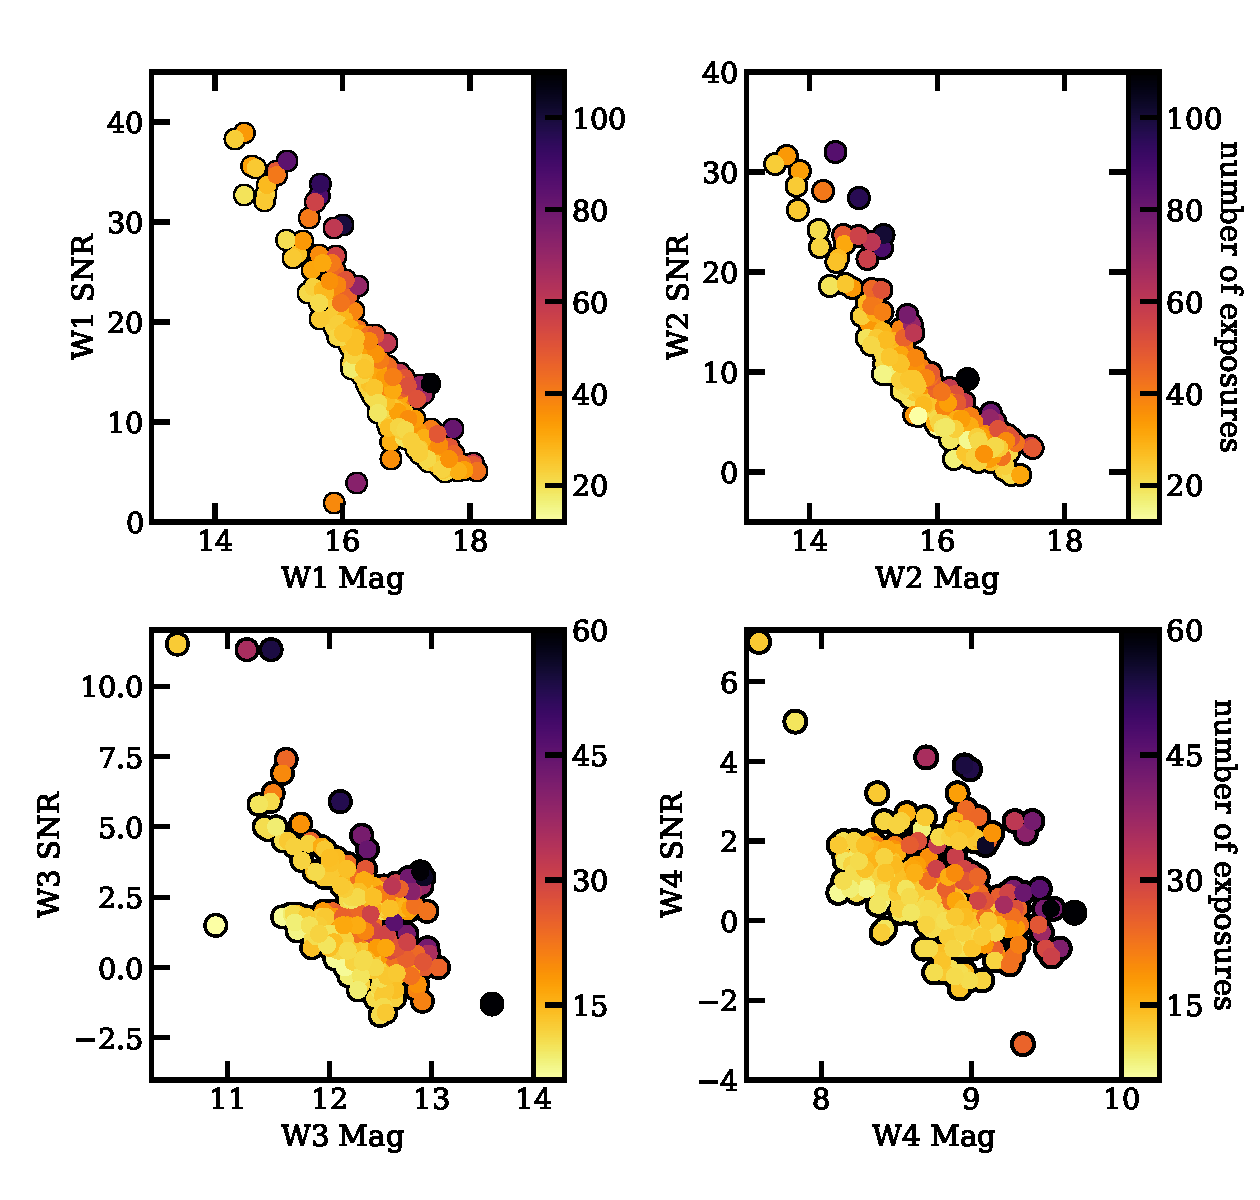
\includegraphics[width=8.6cm, clip,trim=6mm 6mm 0mm 6mm]
      {/cos_pc19a_npr/programs/quasars/highest_z/detections/WISEmag_vs_coverage_2x2_v1.pdf}
      \centering
      \vspace{-14pt}
      \caption[]{WISE W1/2/3/4 magnitude against signal-to-noise, 
        colour coded by w$x$cov the mean coverage depth, in each corresponding band.
      }
      \label{fig:WISEmag_vs_coverage}
    \end{figure}
    
    Table~\ref{tab:mir_detection} gives the detection rates for the
    VH$z$Qs in the MIR WISE W1-4 bands. 
    \begin{table}
      \begin{tabular}{l r l}
        \hline  \hline
        Selection   & number detected (\%) \\
        \hline  
        W1 SNR $> 2.0$   &  275  (64.9) \\
        W2 SNR $> 2.0$   &   255 (60.1) \\
        W1 \&\& W2 SNR $> 2.0$  &  \\
        W3 SNR $> 2.0$   &  99    (23.3) \\
        W4 SNR $> 2.0$   &  29    (6.8) \\
        Any W1/2/3/4 SNR $>2.0$ & \\
        W1/2 SNR $< 2.0$ $\land$ W3 SNR $>2.0$ & \\
        \hline  \hline
      \end{tabular}
      \caption{ATLAS \citet{Shanks2015}; }
      \label{tab:mir_detection}
    \end{table}
    
    \begin{figure}
      %% trim=l b r t
      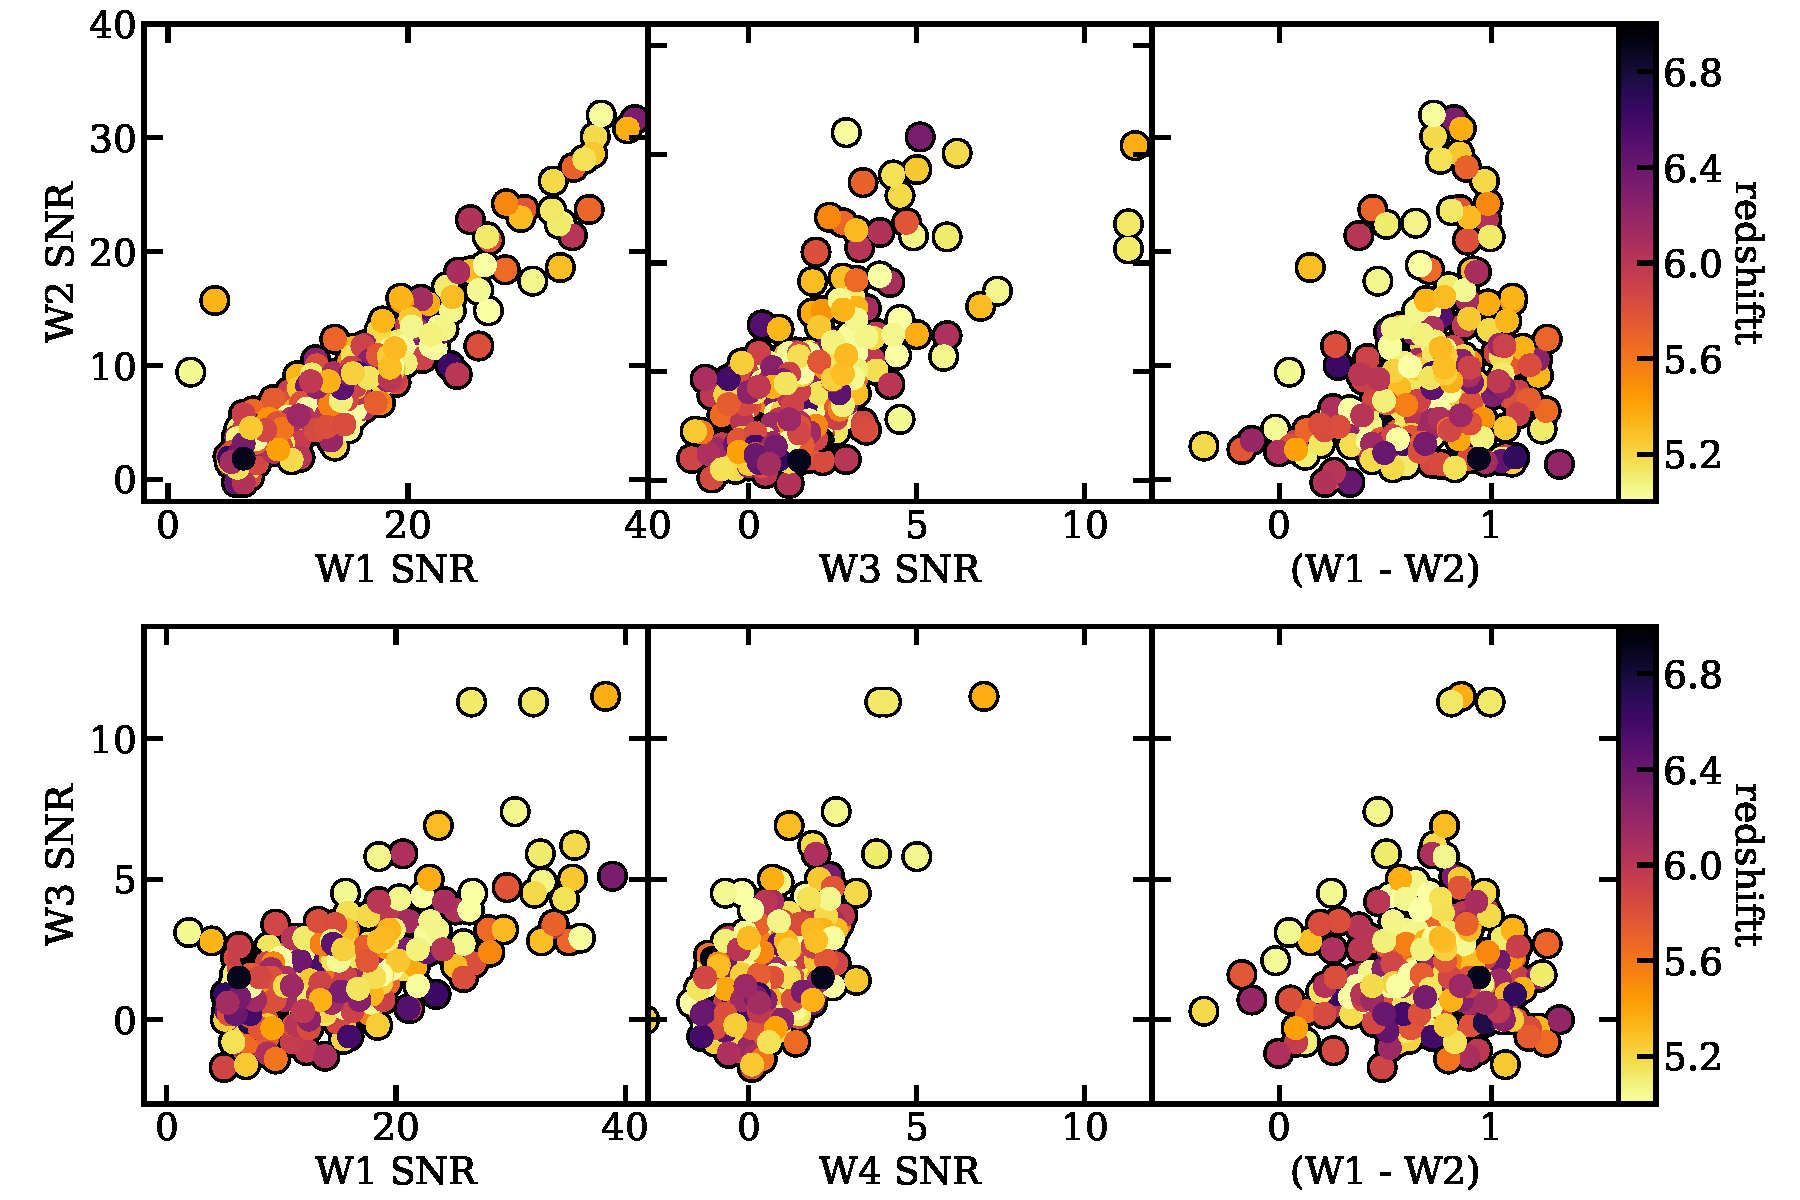
\includegraphics[width=8.6cm, clip,trim=2mm 0mm 2mm 0mm]
      {/cos_pc19a_npr/programs/quasars/highest_z/detections/WISEsnrW1W2W3W4_2by3_v1.pdf}
      \centering
      \vspace{-14pt}
      \caption[]{WISE signal-to-noise measures for the four bands, as well
        as for (W1-W2) colour.  The points are colour coded by redshift.}
      \label{fig:WISEmag_vs_coverage}
    \end{figure}

    \citet{Blain2013} 

    Recently, \citet{Assef2018} released two large catalogues of AGN 
    candidates identified across 30,000 deg$^2$ of extragalactic sky 
    from the WISE AllWISE Data Release. The ``R90'' catalogue, is 
    contains 4.5M AGN candidates at 90\% reliability (and $\approx$150 
    AGN candidates per deg$^2$) while the ``C75'' catalog 
    consists of 20.9M AGN candidates at 75\% completeness (and 
    ($\approx$700 AGN candidates per deg$^2$).  Crossmatching 
    out catalogue of 424 VH$z$Qs with these catalogues, produces 
    42 matches with	the R90 sample and 98 matches with the C75 sample. 
    Both catalogues unsurprisingly match to the ultraluminous quasar 
    SDSS J0100+2802 \citep{Wu2015} while the C75, but not the R90 catalogue 
    mathes to ULAS J1120+0641 \citep{Mortlock2011}. Neither catalogue 
    matches J1342+0928 \citep{Banados2018}. 

    %\subsubsection{
    Very High-$z$ Quasars Detected in WISE W3 and W4.


    \begin{figure}
      \centering
      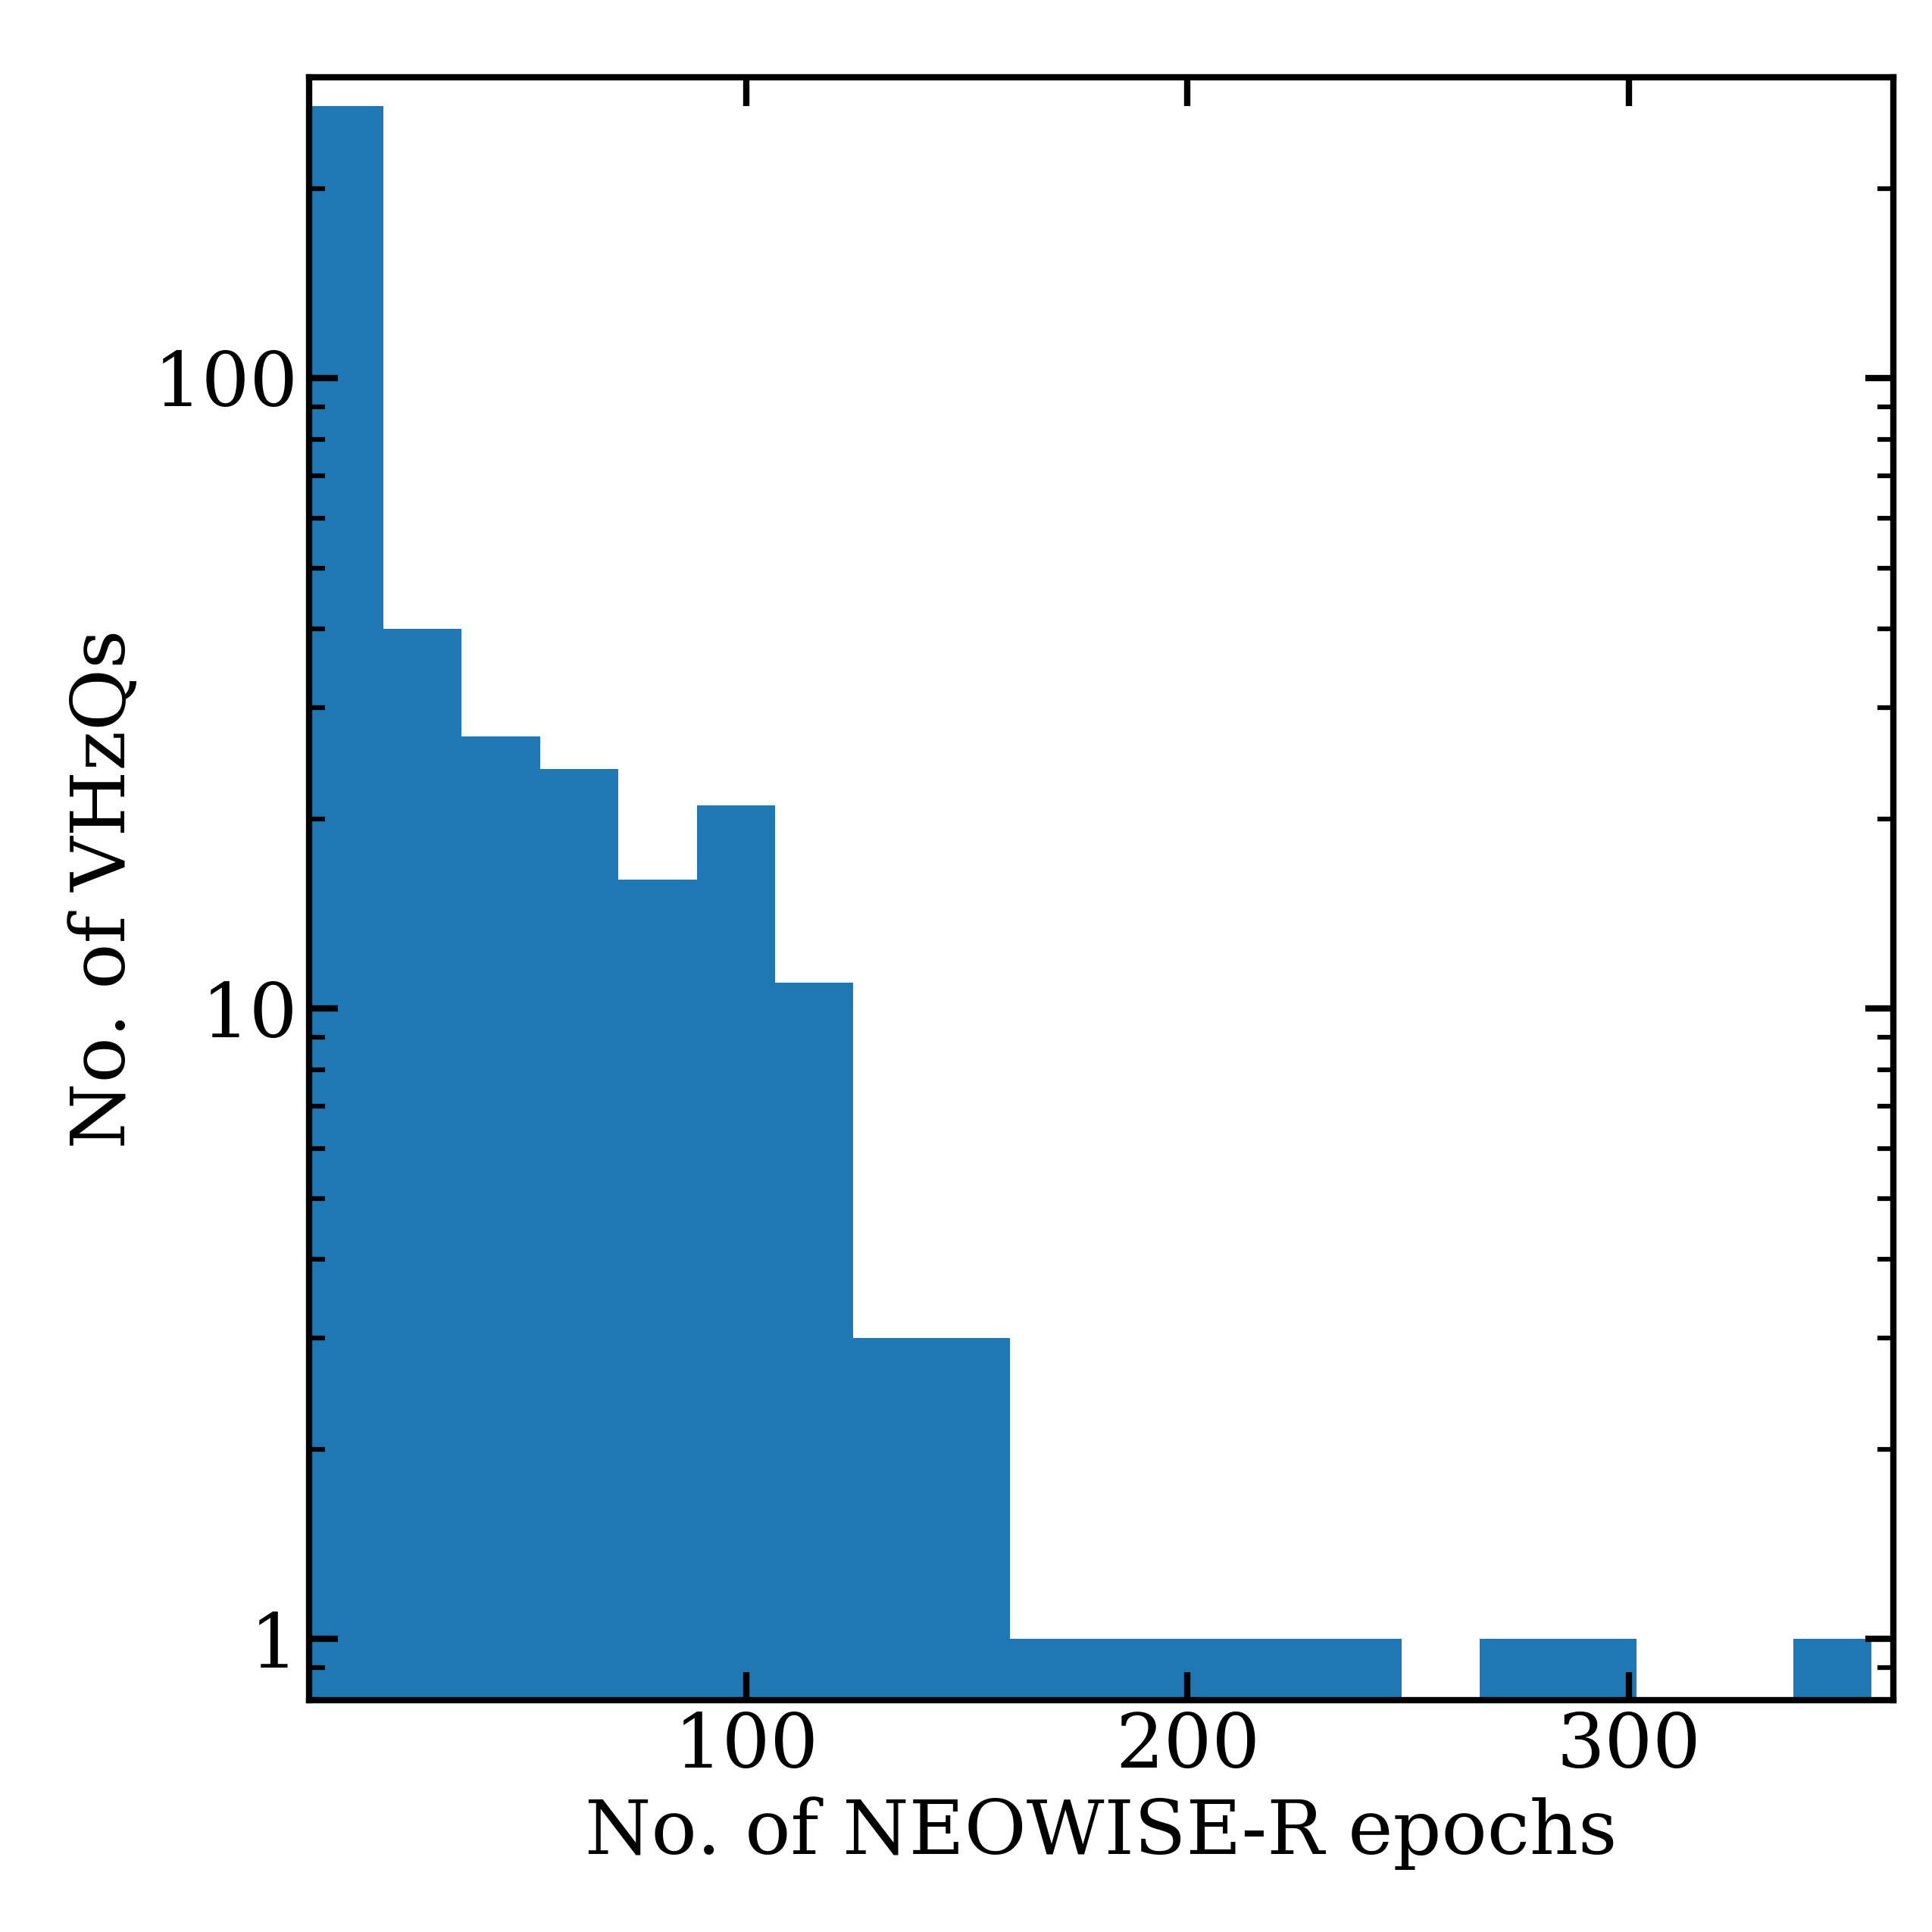
\includegraphics[width=8.5cm]
      {/cos_pc19a_npr/programs/quasars/highest_z/MIR_LCs/NEOWISER_LC_histogramlog_20180827.png}
      \vspace{-16pt}
      \caption[]
      {Histogram showing the number of NEOWISE-R epochs and detections there are for each 
        VH$z$Q.} 
      \label{fig:MIR_LC_epochs}
    \end{figure}
    
\subsection{Variability}
VH$z$Qs, if accreting at, or above the Eddington Limit, might well have have large values of changing mass accretion rate, $\ddot{m_{\rm accr}}$. A consequence of this would be that these quasar exhibit signs of variability, most likely showing up in their UV/optical rest-frame spectra. We look for evidence of this variability signature in the NIR and MIR light-curves of the VH$z$Qs. As a guide, \civ enters the $Y$-band at redshift $z$=5.32 and exits at $z$=5.99, and enters the $J$-band at redshift $z=6.55$ and exits at $z$=7.57. \mgii enters the $H$-band at redshift $z=4.33$ and exits at $z=5.37$ and enters the $K$-band at redshift $z=6.25$ and exits at $7.50$.

Using the extended datasets described in Section~\ref{sec:NIR_data} and~\ref{sec:NIR_SQL}, we 

\begin{figure}
  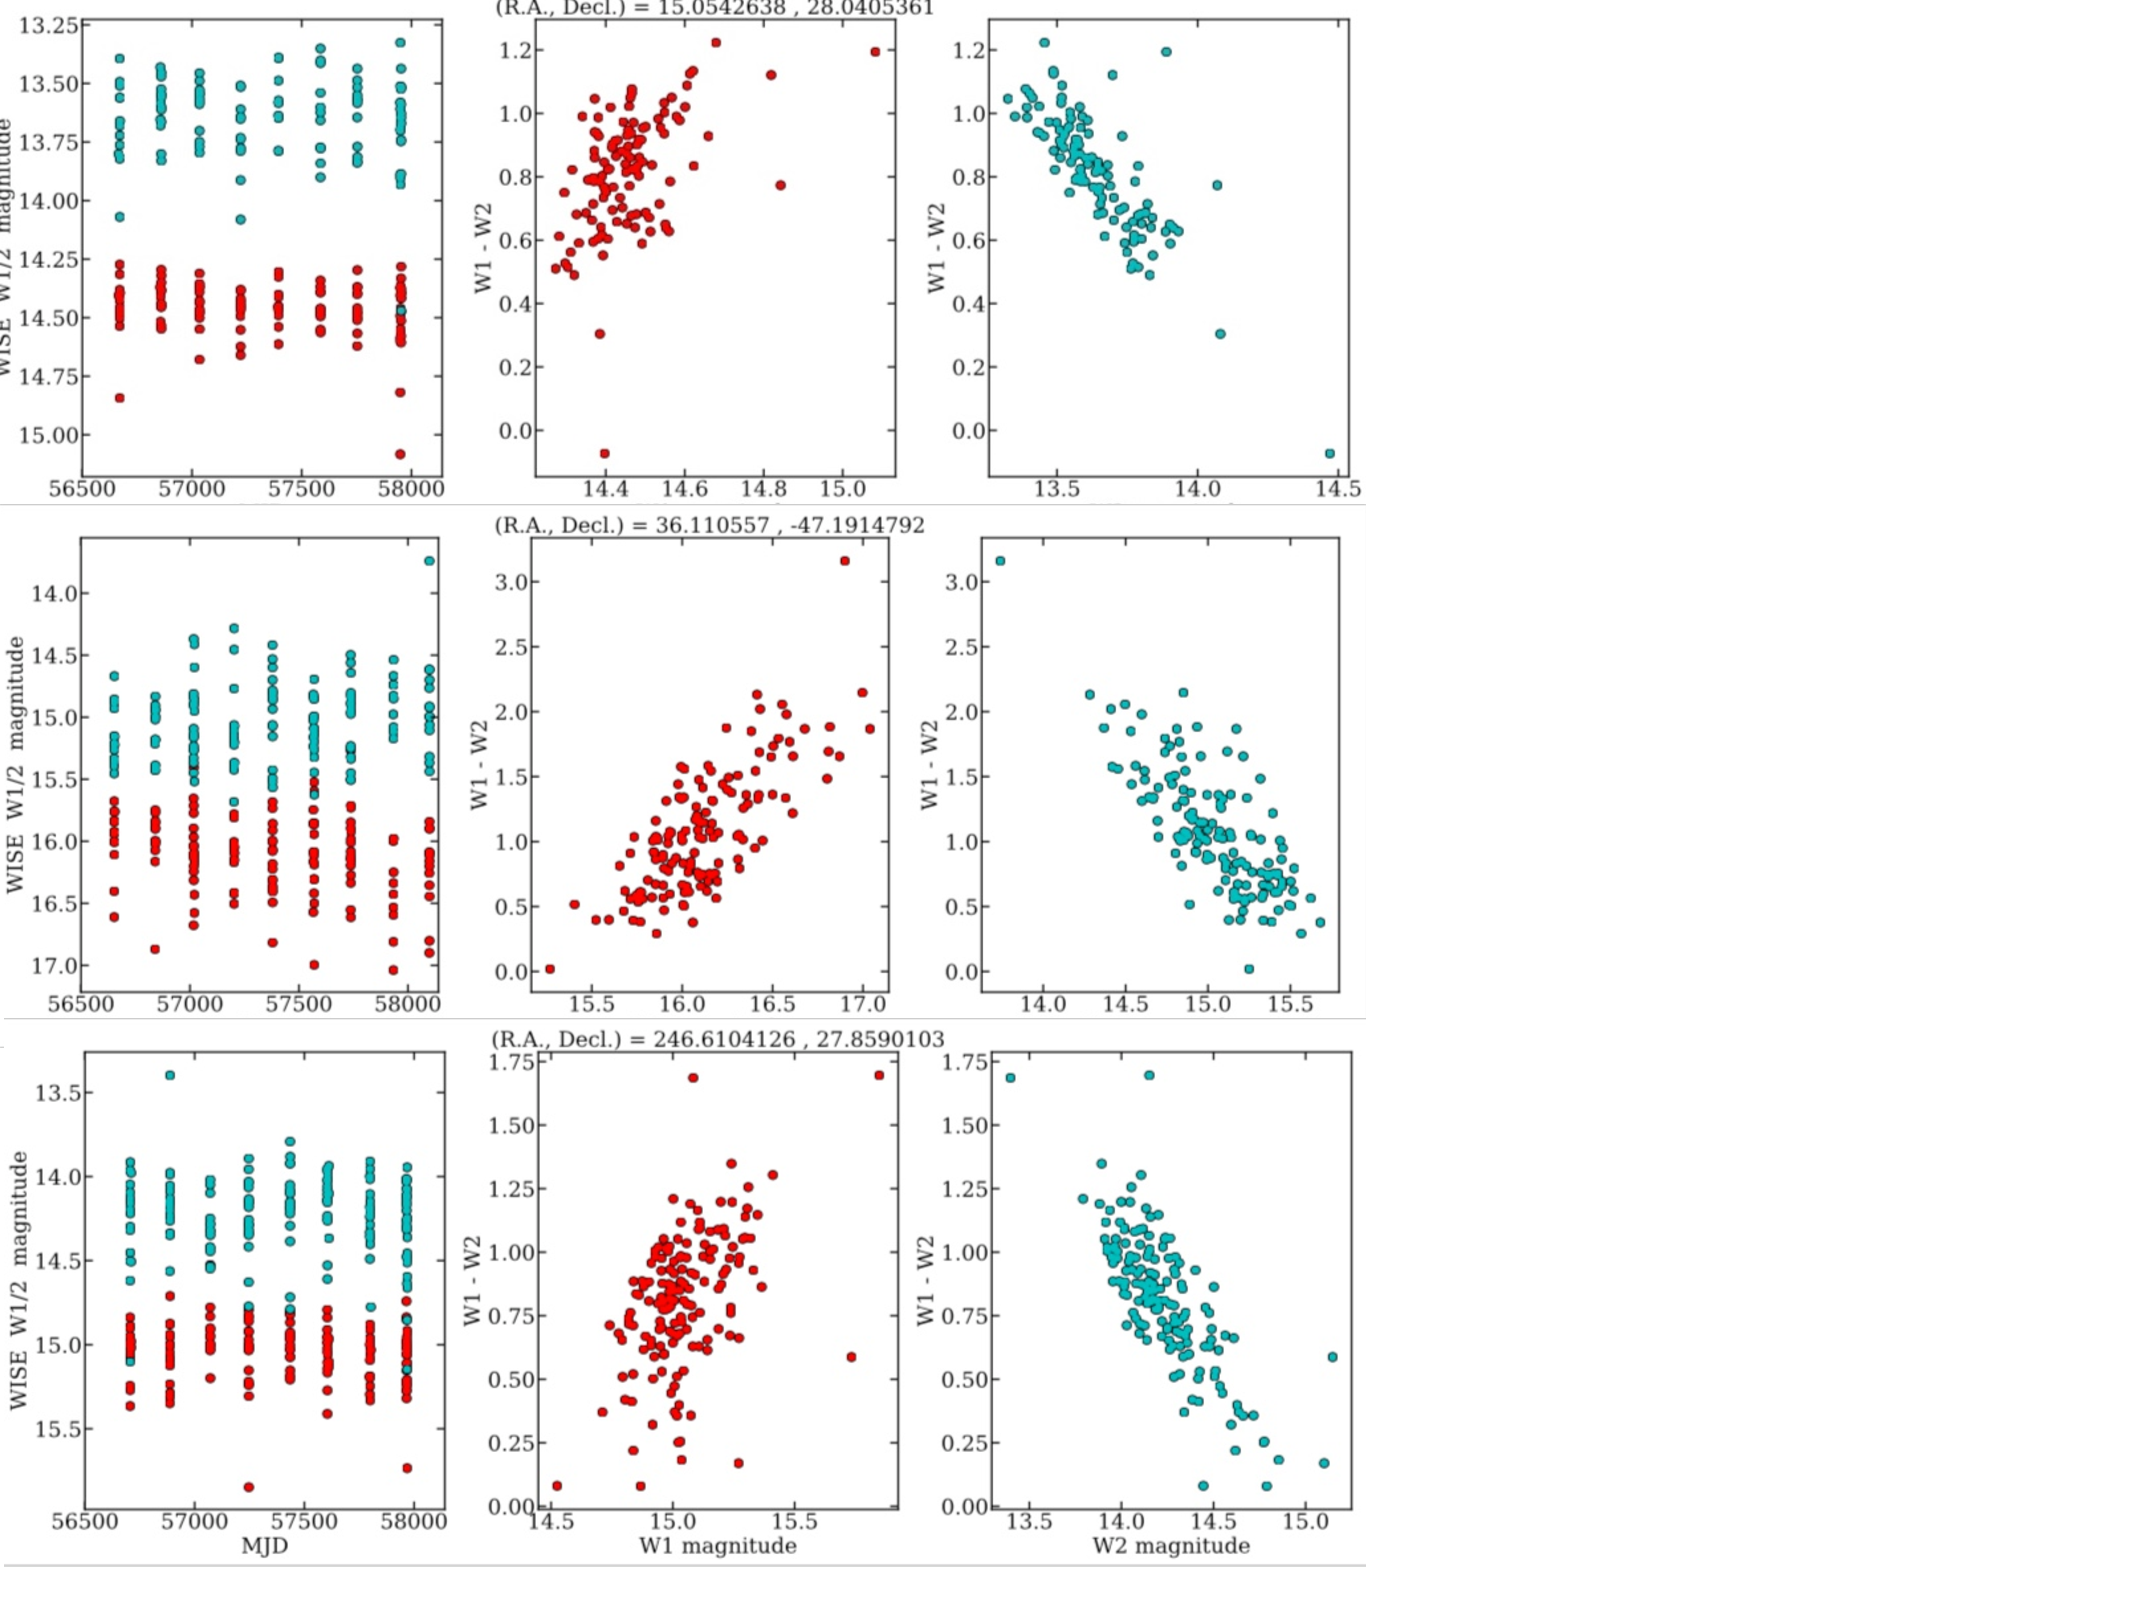
\includegraphics[width=8.5cm]
  {/cos_pc19a_npr/programs/quasars/highest_z/MIR_LCs/three_MIR_LC_egs_20180827.pdf}
  \centering
  \caption[]
  {Here we show the MIR NEOWISE-R for J0100+2802 \citep{Wu2015}, J0224-4711 and  J1626+2751. 
    Red points are the W1 band; cyan points the W2 band.} 
  \label{fig::MIR_LC_3egs}
\end{figure}

Figure~\ref{fig:MIR_LC_epochs} gives the number of NEOWISE-R epochs and detections there are for each VH$z$Q, while 
Figure~\ref{fig:MIR_LC_3egs} presents three examples of the MIR lighcurves and associated colour changes. Here we show 
J0100+2802 \citep{Wu2015}, J0224-4711 and  J1626+2751. 


\subsection{Colours}
Currently, very high-redshift quasars are identified by their morphology, flux and colours in 
optical and infrared imaging data \citet{Fan1999, Mortlock2012}
Quasars are generally selected to be point sources, but 
be outliers from the stellar locus in colour space. For VH$z$Qs, the main technique is to 
look for objects with extreme optical-to-near-infrared colours
The lack of proper motion can also help identified quasars \citep[e.g.][]{Lang2009}. 


Pellentesque vel elit neque, in interdum lacus. Quisque sodales, nunc et luctus convallis, nisl dui luctus dui, at congue urna velit a nisl. Ut sit amet sapien a risus dapibus sagittis. Cras sed ultricies erat. Donec id metus sed urna lacinia convallis vel sed enim. Proin nisi libero, ornare vel bibendum eu, sollicitudin sed leo. Cras tincidunt aliquet ultricies. Cras pretium velit leo, in malesuada enim. Duis sagittis ultricies interdum. Proin sit amet sem nec metus feugiat pharetra.

Figure~\ref{fig:Opt_colourredshift} presents the optical
colour-redshift trends for Late Type M/L/T dwarfs and the VH$z$Qs.

\begin{figure*}
   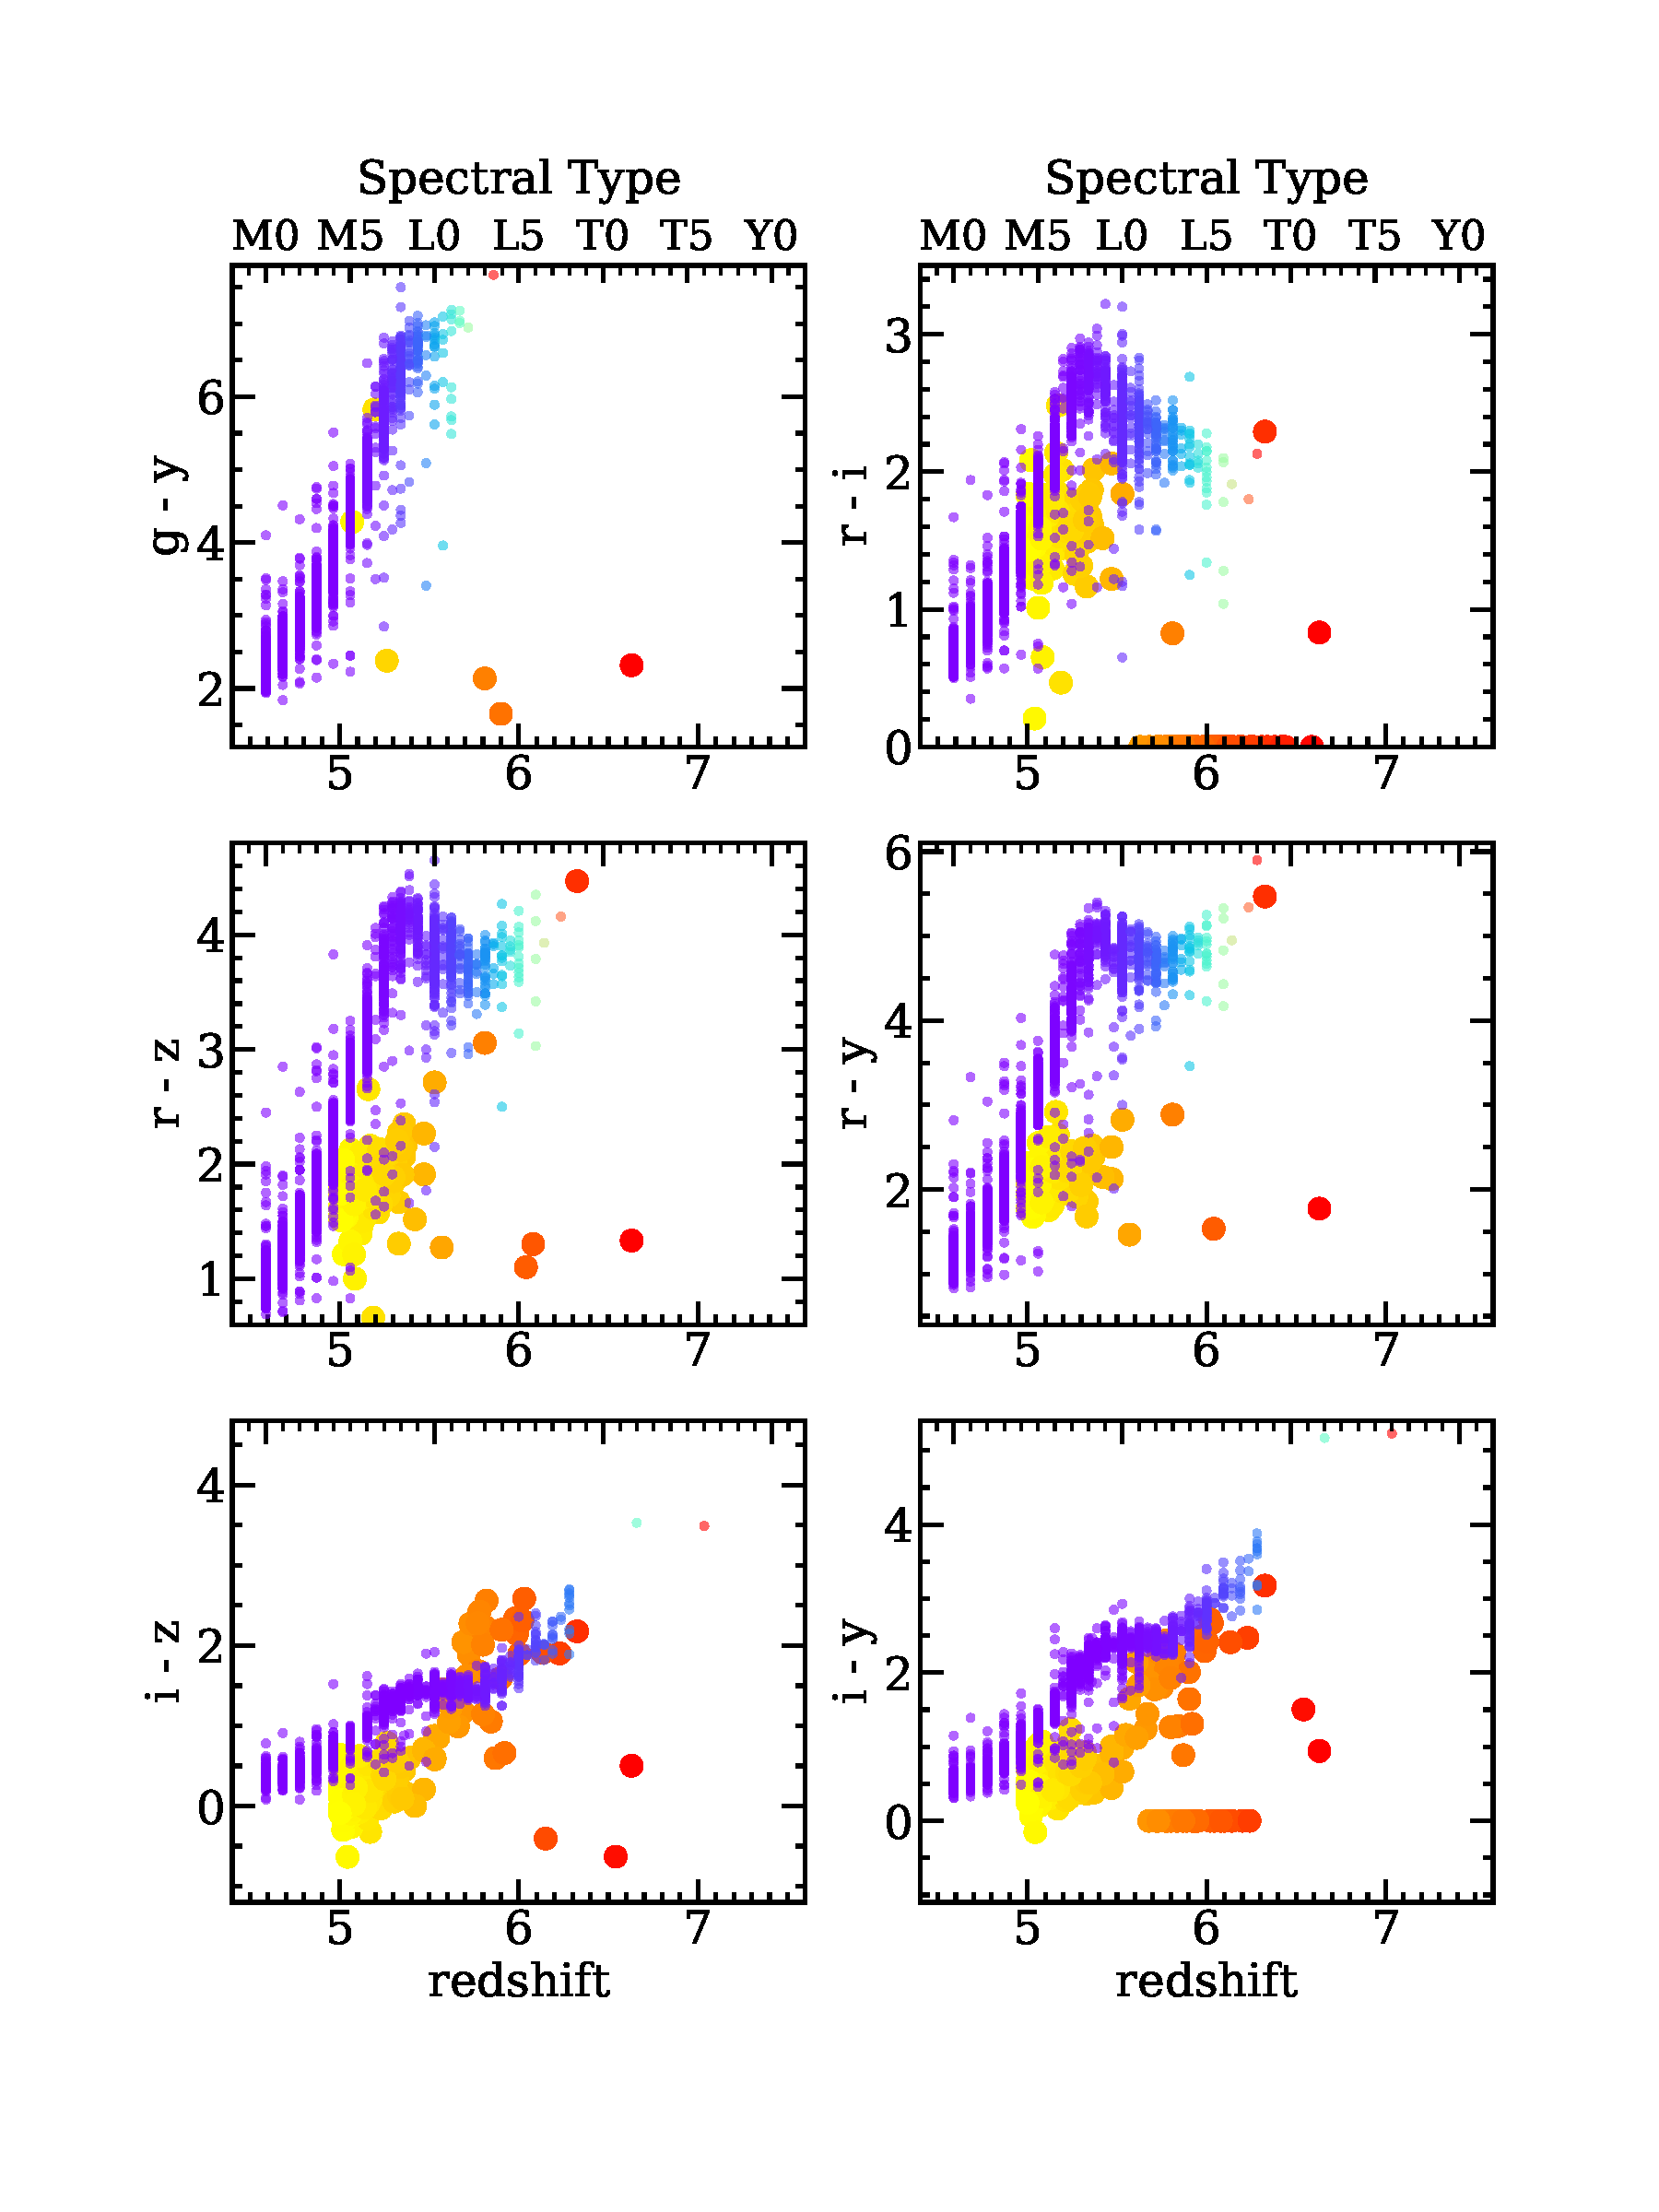
\includegraphics[width=18.0cm]
   {/cos_pc19a_npr/programs/quasars/highest_z/color_redshift/SpecType_vs_Optcolors_20180704.pdf}
   \centering
   \caption[]
   {Optical colour vs. spectral type and redshift for Late Type M/L/T dwarfs and the VH$z$Qs.
     The stars are M, L, and T dwarfs from the \citet{Best2018} PS1-detected catalog.  
   {\it N.B. Trying to look as good as Fig.~5 from Best et al. (2018). How does one get 
bigger gaps between subplots??}}
   \label{fig:Opt_colourredshift}
 \end{figure*}

Figure~\ref{fig:Opt_colourredshift} presents the near-infrared 
colour-redshift trends for Late Type M/L/T dwarfs and the VH$z$Qs.
\begin{figure*}
   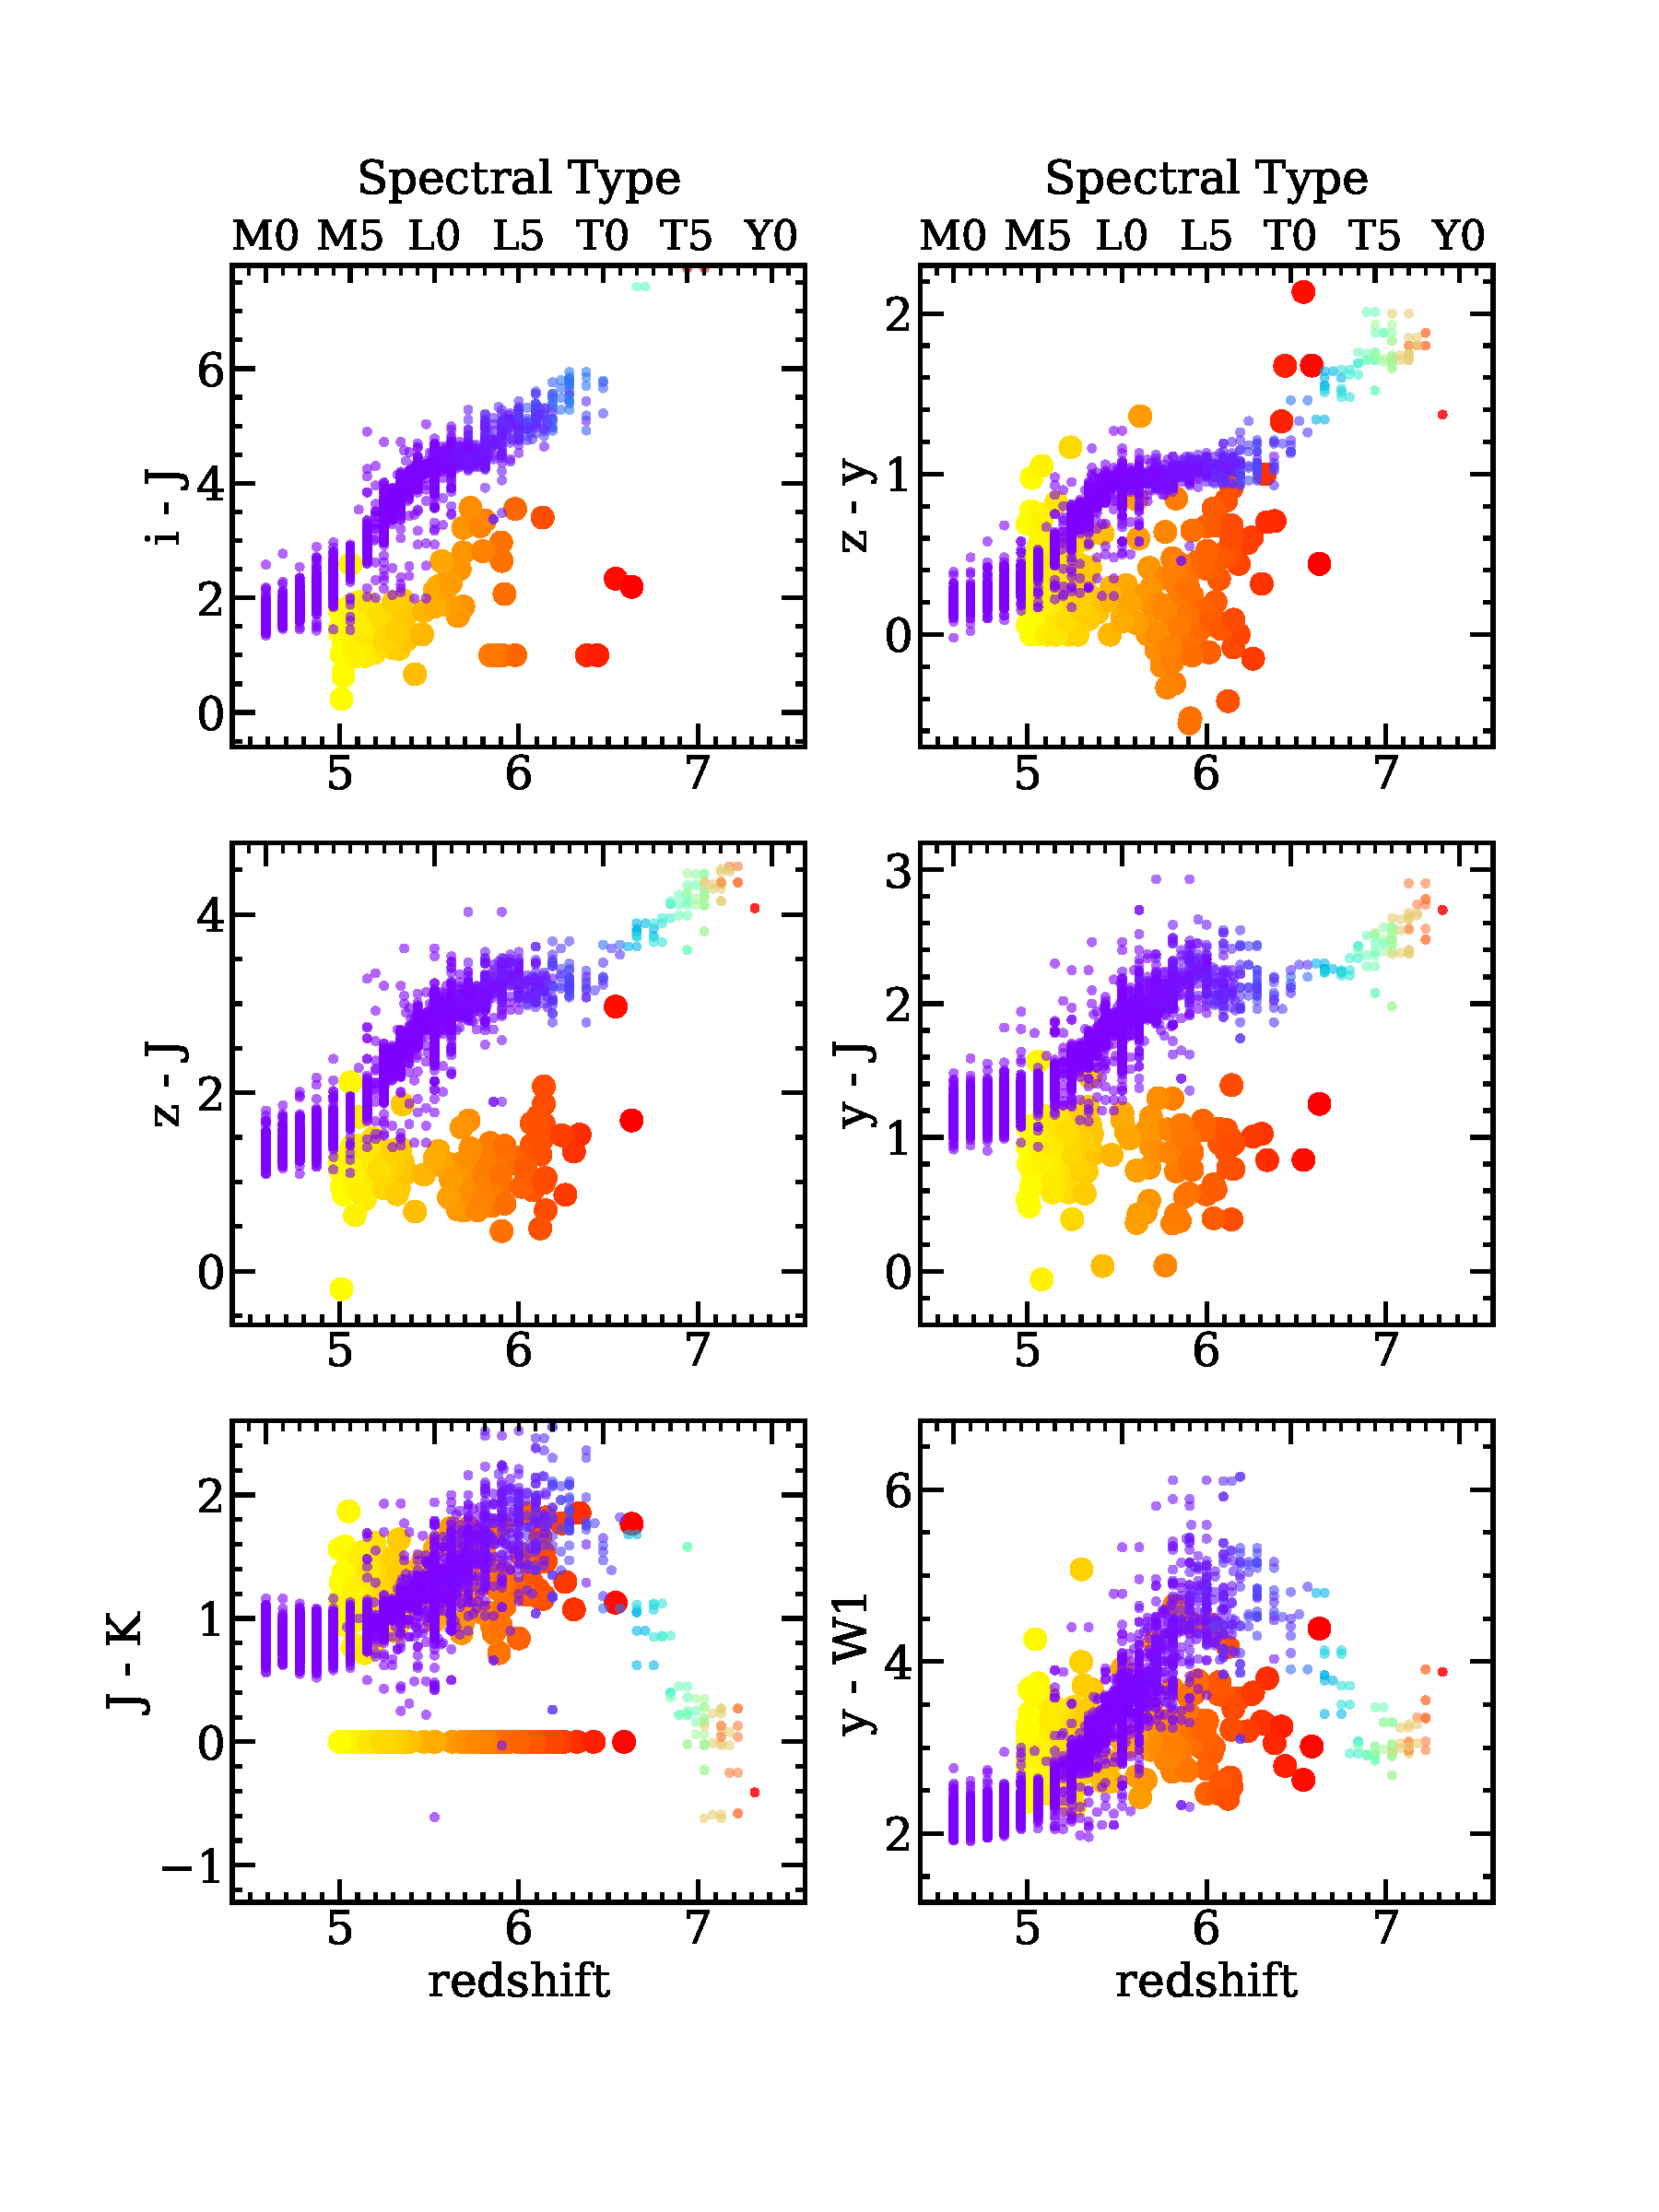
\includegraphics[width=18.0cm]
   {/cos_pc19a_npr/programs/quasars/highest_z/color_redshift/SpecType_vs_NIRcolors_20180704.pdf}
  \centering
   \caption[]
   {Infrared colour-spectral type and redshift plots for Late Type M/L/T dwarfs and the VH$z$Qs.
     {\it NB} I'm really not sure how Best et al. actually get their stellar sequence so clean. 
There are two types of spectral classification,  but restricting it to just SpT\_optn  or SpT\_nir removes
the blue or red end respectively. Hmmm....}
   \label{fig:SpecType_vs_NIRcolors}
 \end{figure*}

\begin{figure*}
   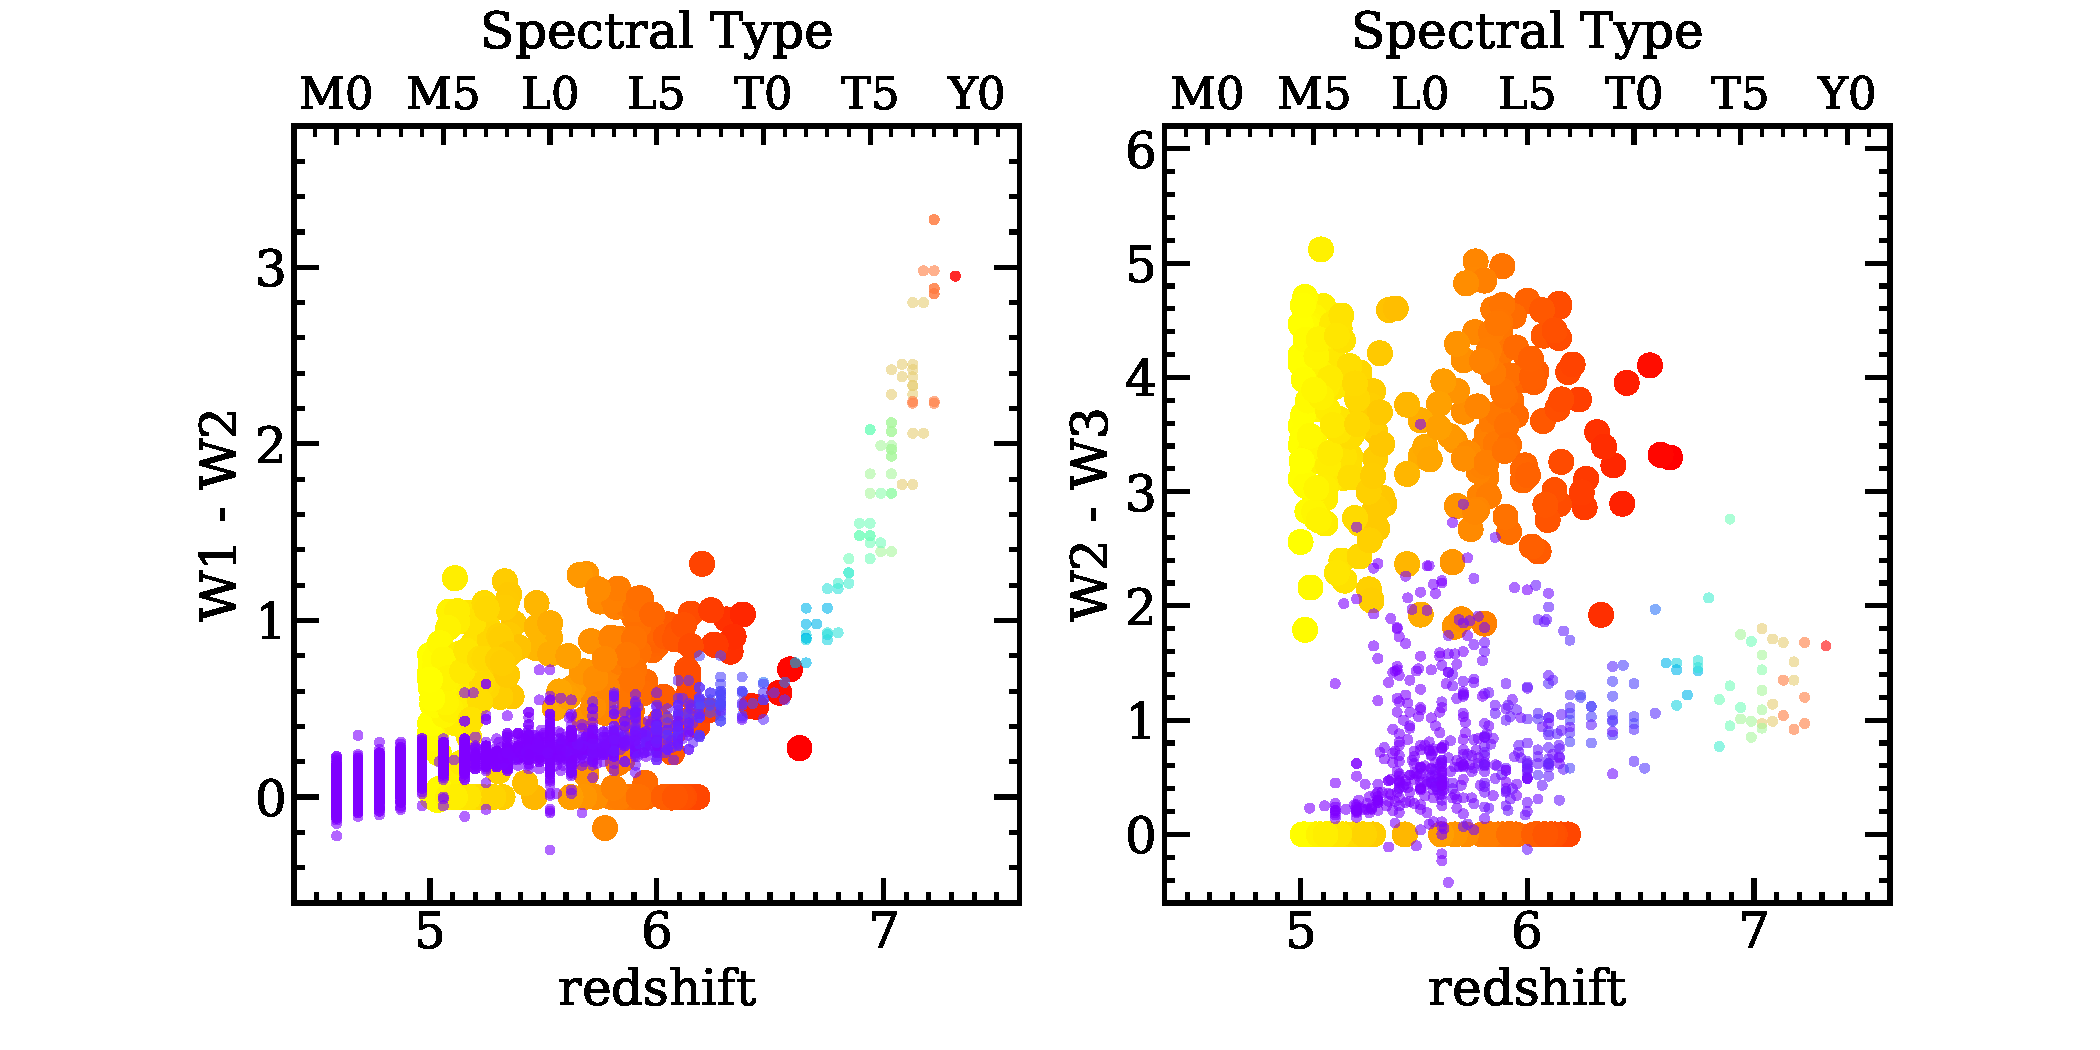
\includegraphics[width=18.0cm]
   {/cos_pc19a_npr/programs/quasars/highest_z/color_redshift/SpecType_vs_W1W2_W2W3colors_20180407.pdf}
  \centering
   \caption[]
   {Infrared colour-spectral type and redshift plots for Late Type M/L/T dwarfs and the VH$z$Qs.
}
   \label{fig:SpecType_vs_W1W2_W2W3colors}
 \end{figure*}




\subsection{L-$z$ Plane}
Having obtained an as-near-to-homogenous set of photometry as we can, 
we are now in a position to calculate the Absolute Magnitudes of the VH$z$Q 
sample and in particulare the absolute magnitude at rest-frame 1450\AA'\, $M_{1450}$, 
which is a key physical quantity and goes directly towards the quasar luminosity 
function and thus the reionization of hydrogen calculation. 

At $z=5.00$, the rest-frame 1450\AA\ emission is redshifted to 8700\AA\ iobserved, 
i.e., in the $z$-band, while at 

\begin{figure*}
  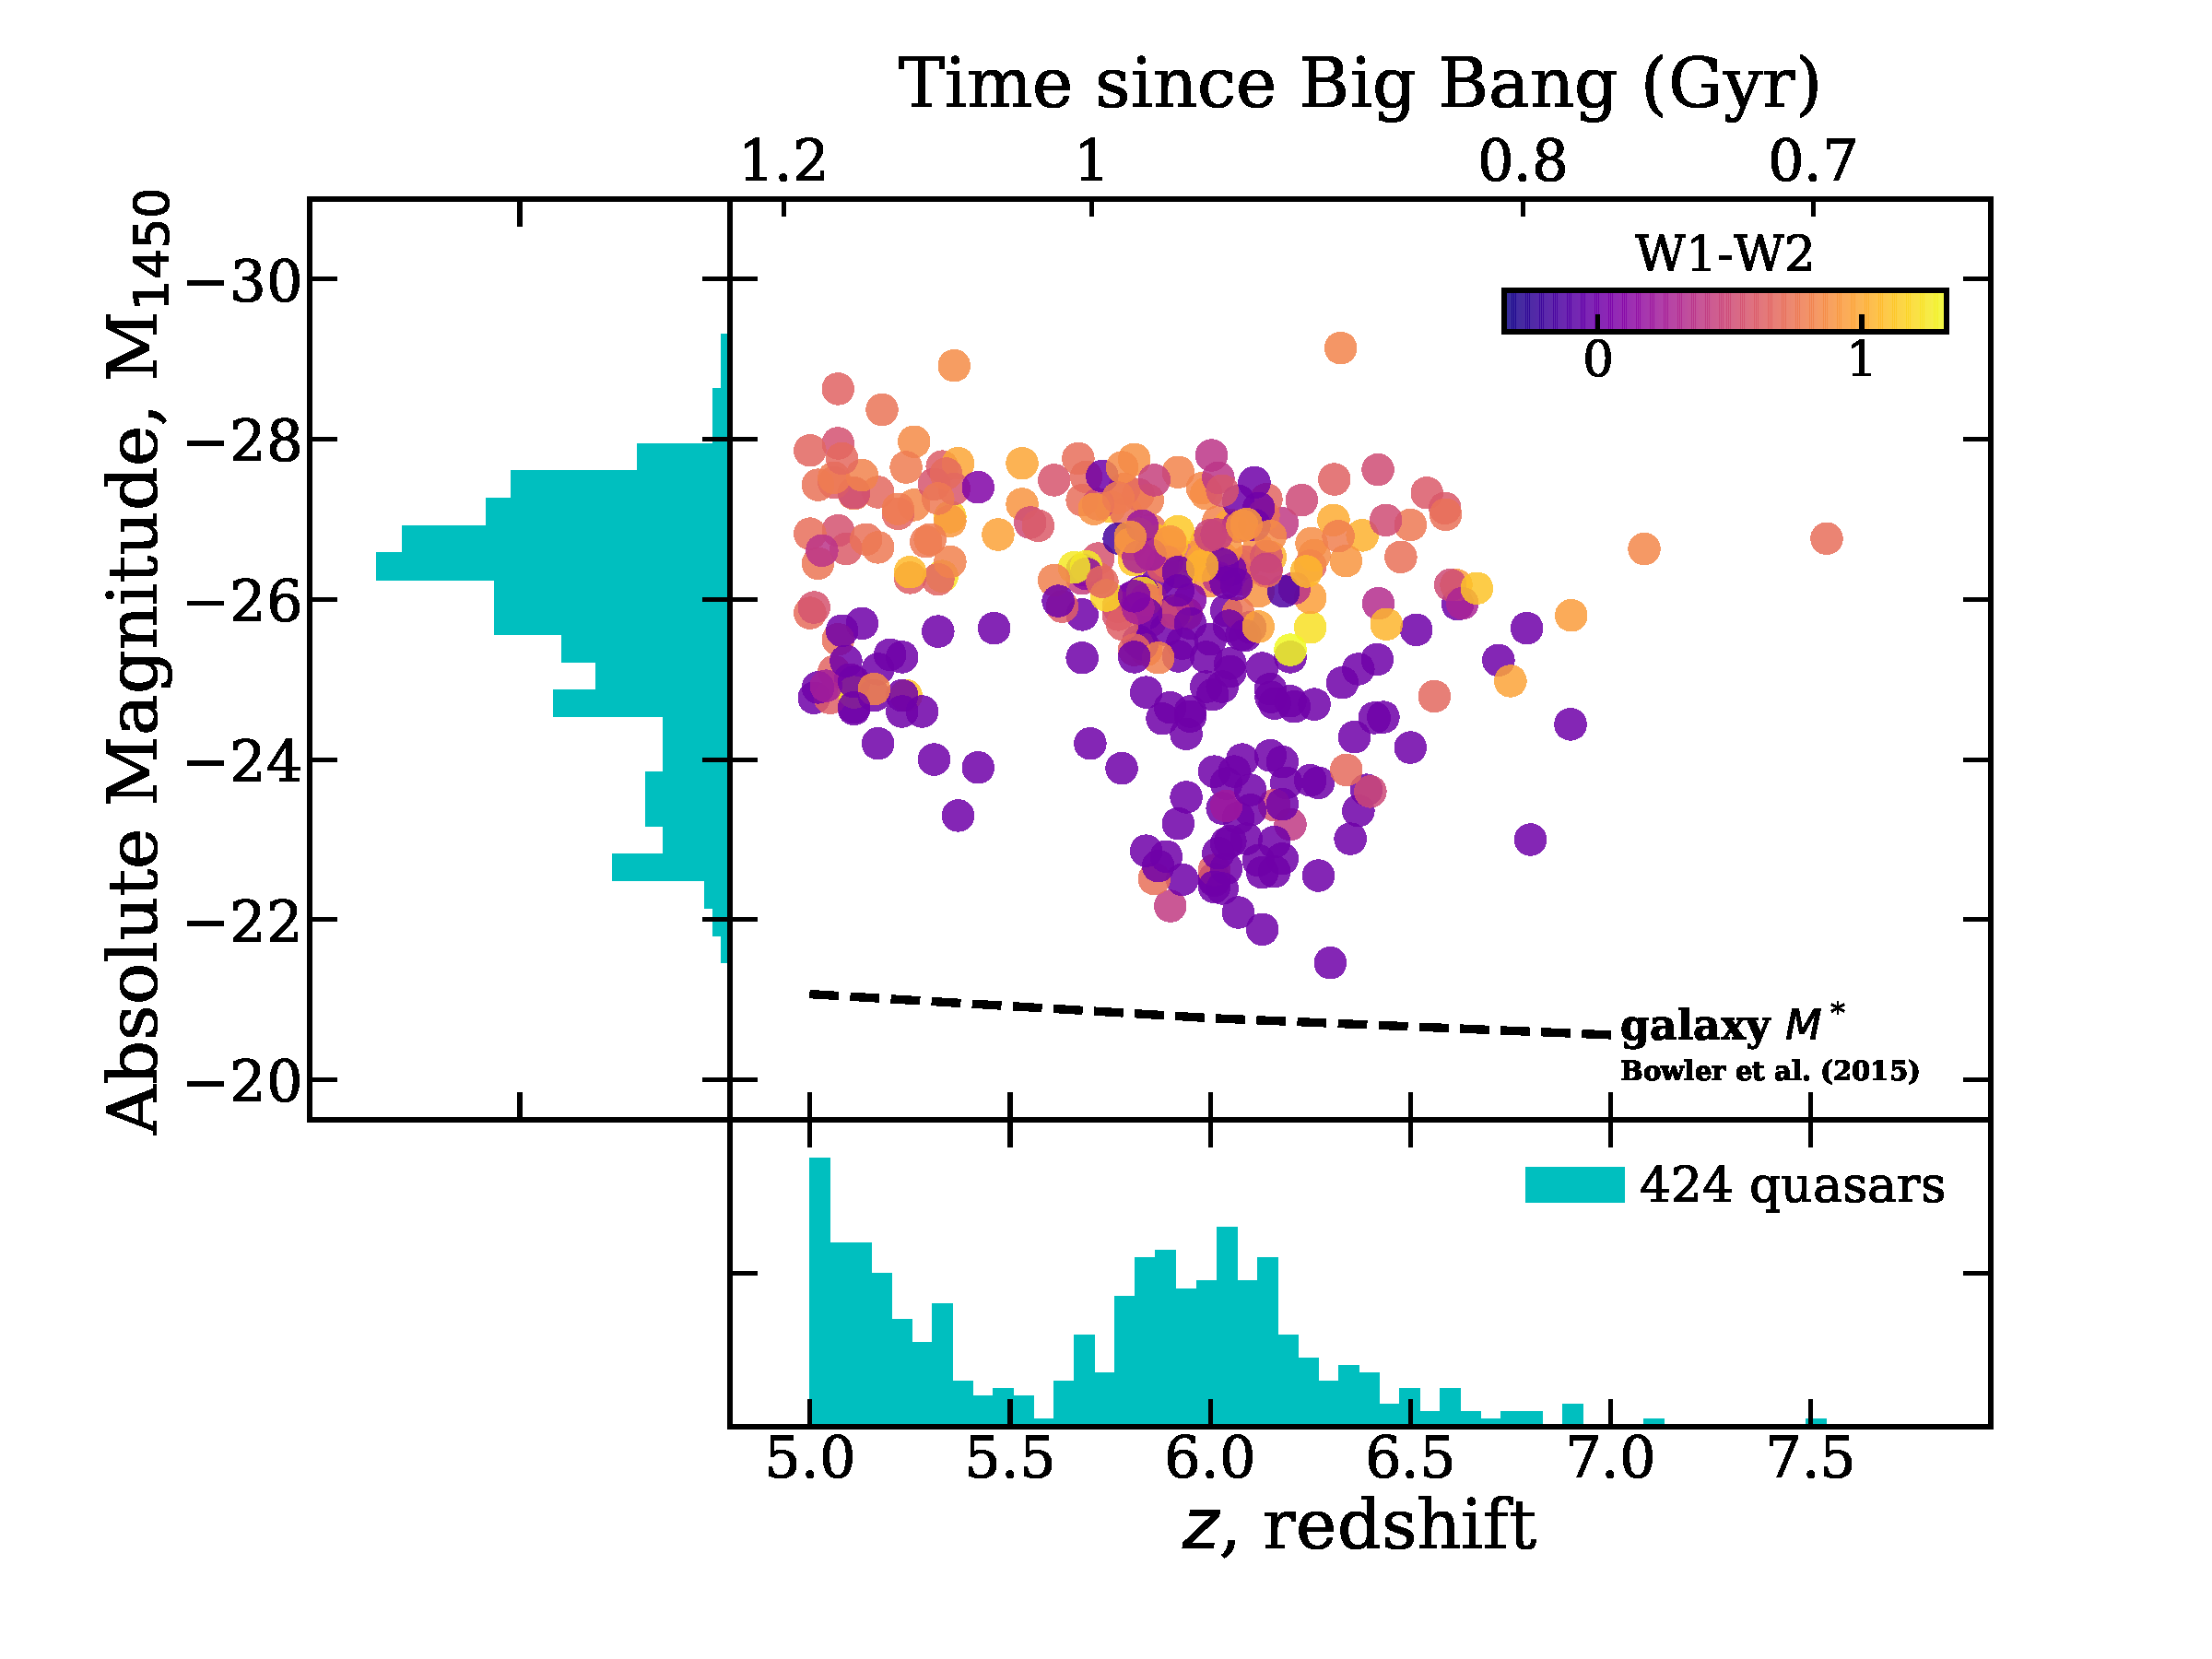
\includegraphics[width=18.0cm]
  {/cos_pc19a_npr/programs/quasars/highest_z/Lz/VHzQ_Lz_20180702.pdf}
  \centering
  \caption[]
  {The spectral bands used by different survey telescopes and that are relevant here.}
  \label{fig:Lz}
\end{figure*}





\subsection{SEDs and Dust properties of the VH$z$Qs}
There are a range of IR SEDs e.g. \citet{Mullaney2013} etc. etc. etc. 
However, they are, for our purposes all roughly the same. 

\begin{figure*}
  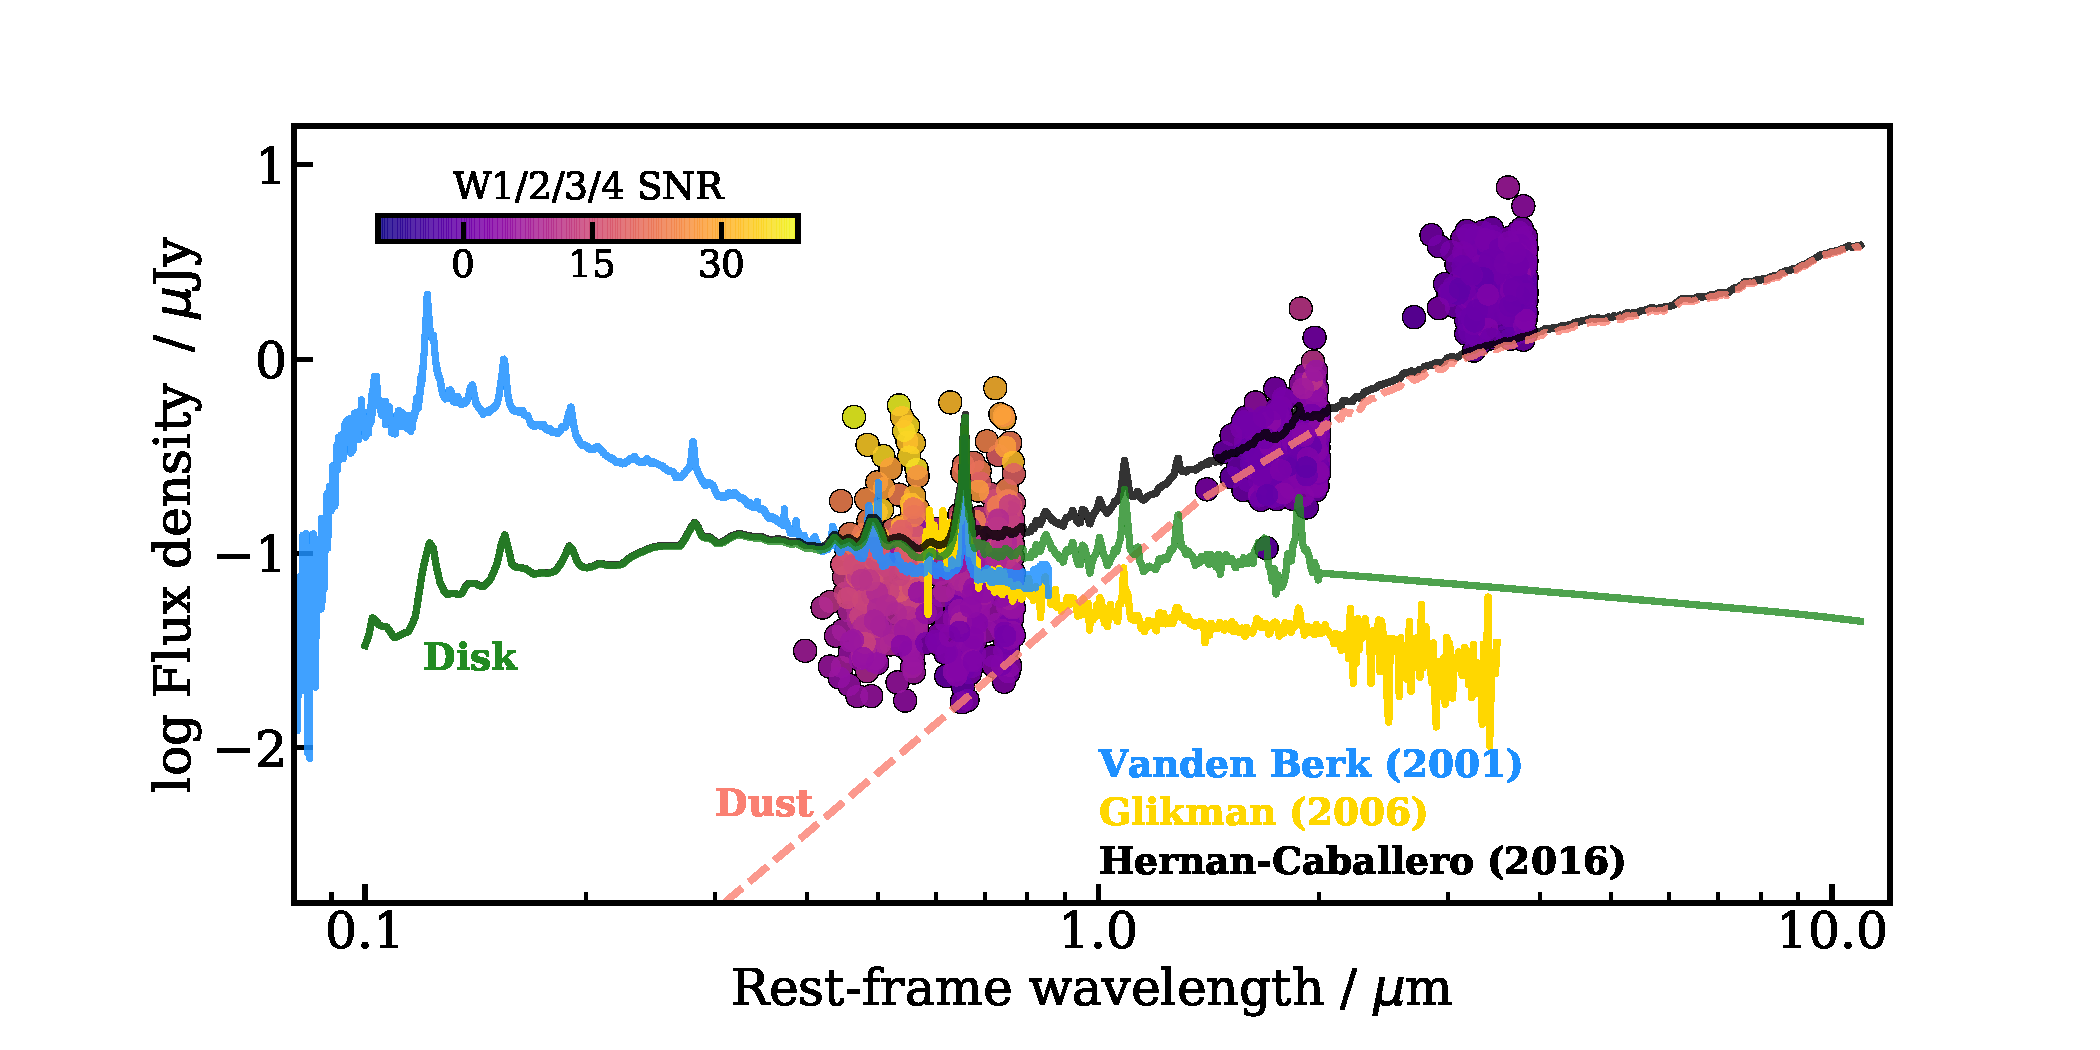
\includegraphics[width=18.0cm]
  {/cos_pc19a_npr/programs/quasars/highest_z/SEDs/RestWavelength_flux_20180702.pdf}
  \centering
  \caption[]
  {The rest-frame properties of the VH$z$Qs. }
  \label{fig:RestWavelength_SEDs}
\end{figure*}



%%%%%%%%%%%%%%%%%%%%%%%%%%%%%%%%%%%%%%%%%%%%%%%%%%%%%%%%%%%%%%%%%%
%%%%%%%%%%%%%%%%%%%%%%%%%%%%%%%%%%%%%%%%%%%%%%%%%%%%%%%%%%%%%%%%%%
%%
%%  S E C T I O  N   7         S E C T I O  N   7           S E C T I O  N   7       S E C T I O  N   7
%%  S E C T I O  N   7         S E C T I O  N   7           S E C T I O  N   7       S E C T I O  N   7
%%  S E C T I O  N   7         S E C T I O  N   7           S E C T I O  N   7       S E C T I O  N   7
%%
%%%%%%%%%%%%%%%%%%%%%%%%%%%%%%%%%%%%%%%%%%%%%%%%%%%%%%%%%%%%%%%%%%
%%%%%%%%%%%%%%%%%%%%%%%%%%%%%%%%%%%%%%%%%%%%%%%%%%%%%%%%%%%%%%%%%%
\section{Discussion and Conclusions}
\label{sec:conclusions}
In this study, we have, for the first time, ompiled the list of all
$z>5$ spectroscopically confirmed quasars. We have assemble the NIR
($y/Y, J, H, K/K_{s}$) and MIR (WISE W1/2/3/4) photometry for these
objects, given their detection rates and SEDs. We find that: 

%%
We can gain a good appreciation for what these missions will discover
by collating the datasets we currently have. 

\begin{itemize}
    \item Lorem ipsum dolor sit amet, consectetur adipiscing
      elit. Aliquam porta sodales est, vel cursus risus porta non. Vivamus
      vel pretium velit. Sed fringilla suscipit felis, nec iaculis lacus
      convallis ac. 
    \item Fusce pellentesque condimentum dolor, quis vehicula
      tortor hendrerit sed. Class aptent taciti sociosqu ad litora torquent
      per conubia nostra, per inceptos himenaeos. Etiam interdum tristique
      diam eu blandit. Donec in lacinia libero.
    \item Sed elit massa, eleifend non sodales a, commodo ut felis. Sed id
      pretium felis. Vestibulum et turpis vitae quam aliquam convallis. Sed
      id ligula eu nulla ultrices tempus. Phasellus mattis erat quis metus
      dignissim malesuada. Nulla tincidunt quam volutpat nibh facilisis
      euismod. Cras vel auctor neque. Nam quis diam risus.
\end{itemize}
Nunc lacus nibh, convallis ac lobortis ut, tempus ac lectus. Maecenas
eu elit massa. Nulla vel lacus lorem. Proin et lobortis
tortor. Phasellus ultrices nisl non enim porttitor dictum. Curabitur
nec nunc ac nibh ornare elementum. Nunc ultrices hendrerit
ultricies. Aliquam dapibus semper est et gravida. Etiam cursus, massa
eget tempor elementum, lectus urna feugiat nisi, eget sagittis.

\subsection*{Author Contributions}   
N.P.R. initiated the project, compiled the list of $z>5.00$ quasars, wrote most of the analysis code, developed the the plotting scripts, and developed and wrote the initial and subsequent drafts of the manuscript.

N.J.G.C. supplied the critical near-infrared expertise and database for which the bulk of the project relies. N.J.G.C. also contributed directly to the writing of the manuscript.


\subsection*{Availability of Data and computer analysis codes} 
All materials, data, code and analysis algorithms are fully 
available at: 
\href{https://github.com/d80b2t/VHzQ}{\tt https://github.com/d80b2t/VHzQ}


\section*{Acknowledgements}
NPR acknowledges support from the STFC and the Ernest Rutherford Fellowship scheme. 

We thank Mike Read at the ROE WFAU for help with the WFCAM Science Archiv (WSA), and 
also the VISTA Science Archive (VSA). We thank Bernie Shiao at STScI for help with the Pan-STARRS1 DR1 CasJobs interface. 

This paper heavily used \href{http://www.star.bris.ac.uk/~mbt/topcat/}{TOPCAT} (v4.4)
\citep[][]{Taylor2005, Taylor2011}.
%%
This research made use of \href{http://www.astropy.org}{\tt Astropy}, 
a community-developed core Python package for Astronomy 
\citep{AstropyCollaboration2013, AstropyCollaboration2018}. 

The Pan-STARRS1 Surveys (PS1) and the PS1 public science archive have
been made possible through contributions by the Institute for
Astronomy, the University of Hawaii, the Pan-STARRS Project Office,
the Max-Planck Society and its participating institutes, the Max
Planck Institute for Astronomy, Heidelberg and the Max Planck
Institute for Extraterrestrial Physics, Garching, The Johns Hopkins
University, Durham University, the University of Edinburgh, the
Queen's University Belfast, the Harvard-Smithsonian Center for
Astrophysics, the Las Cumbres Observatory Global Telescope Network
Incorporated, the National Central University of Taiwan, the Space
Telescope Science Institute, the National Aeronautics and Space
Administration under Grant No. NNX08AR22G issued through the Planetary
Science Division of the NASA Science Mission Directorate, the National
Science Foundation Grant No. AST-1238877, the University of Maryland,
Eotvos Lorand University (ELTE), the Los Alamos National Laboratory,
and the Gordon and Betty Moore Foundation.

This project used data obtained with the Dark Energy Camera (DECam)
and the NOAO Data Lab, The Data Lab is operated by the National
Optical Astronomy Observatory, the national center for ground-based
nighttime astronomy in the United States operated by the Association
of Universities for Research in Astronomy (AURA) under cooperative
agreement with the National Science Foundation.

This publication makes use of data products from the Wide-field
Infrared Survey Explorer, which is a joint project of the University
of California, Los Angeles, and the Jet Propulsion
Laboratory/California Institute of Technology, and NEOWISE, which is a
project of the Jet Propulsion Laboratory/California Institute of
Technology. WISE and NEOWISE are funded by the National Aeronautics
and Space Administration.

CasJobs was originally developed by the Johns Hopkins University/
Sloan Digital Sky Survey (JHU/SDSS) team. With their permission, MAST
used version 3.5.16 to construct CasJobs-based tools for GALEX,
Kepler, the Hubble Source Catalog, and PanSTARRS.

This research has made use of the SVO Filter Profile Service
(http://svo2.cab.inta-csic.es/theory/fps/) supported from the Spanish
MINECO through grant AyA2014-55216 
%%
The SVO Filter Profile Service\footnote{Rodrigo, C., Solano, E., Bayo, A. http://ivoa.net/documents/Notes/SVOFPS/index.html}
describes the Spanish VO Filter Profile Service. 
The Filter Profile Service Access Protocol. Rodrigo, C., Solano, E. http://ivoa.net/documents/Notes/SVOFPSDAL/index.html

\newpage

\appendix
\section{Filter Curves} 
FRom the SVO Filter Profile Service\footnote{http://svo2.cab.inta-csic.es/svo/theory/fps/}.

\section{A. Photometric Bands and Conversions}
    Due to the differing normalizations between the
    SDSS and  UKIDSS photometric systems, certain corrections are required.  To present
    our data in the  purest sense, all the NIR magnitudes from UKIDSS
    (originally AB magnitudes)  were corrected to Vega magnitudes as
    suggested in \citet{Hewett2006}.
    
    Although ULAS magnitudes are reported in terms of Vega and SDSS
    magnitudes are reported in AB terms for the most part whenever an
    optical-NIR color was calculated both magnitudes were left in their
    default term.
    
\begin{table*}
  \begin{center}
   \caption{Adapted from Table 9 of \citet{Peth2011}. 
CTIO/DECam, PanSTARRS/PS1, LSST
%References: www.cfht.hawaii.edu/Instruments/Filters/wircam.html
Filter only values. 
All wavelengths in ${\buildrel _{\circ} \over {\mathrm{A}}}$. 
%%
%%
From \citet{GonzalezFernandez2018} 
$Z_{\rm AB}   -  Z_{\rm Vega}  = 0.502$;  
$Y_{\rm AB}  -  Y_{\rm Vega}    = 0.600 $;
$J_{\rm AB}   -  J_{\rm Vega}    = 0.916  $;
$H_{\rm AB}  -  H_{\rm Vega}    = 1.366 $;
$Ks_{\rm AB}  -  Ks_{\rm Vega}  = 1.827 $;
%%
and the CASU Vega to AB conversions v1.3:: 
	Z,Y,J,H,Ks were: 0.524, 0.618, 0.937, 1.384, 1.839. 
%%
So, $\Delta$(vs. Gonzalez-Fernandez)::
	(11.2,     1.1,    5.4,     1.6,    0.1) millimags. 
$\Delta$(vsCASU v1.3)::
	(-10.8, -16.9, -15.6,  -16.4, -11.9) millimags. 
}
    \setlength{\tabcolsep}{4pt}
     \begin{tabular}{l r r r  c l l}
      %% https://www.gemini.edu/sciops/instruments/magnitudes-and-fluxes
      %% http://wise2.ipac.caltech.edu/docs/release/allsky/expsup/sec4_4h.html#conv2ab
      \hline
      \hline
      Band & $\lambda_{\rm eff}  $ 
              &  $\lambda_{\rm min} $ 
              & $\lambda_{\rm max} $ 
              & W$_{\rm eff}$
              & \multicolumn{2}{c}{AB - Vega  Transformations} \\
      \hline
      % {\it u} & 3551  &  3005 &  4000 &  581 & $u$ = $u_{AB}$ - 0.927 \\
      % {\it u_{\rm LSST}} &	3733 &	3182 &	4082 &	?? \\
       $g_{\rm HSC}$    &  	4633   &     3940     &   5546	&  1460       &    $g_{\rm HSC}$         &$  = g_{\rm AB} + 0.097 $ \\
      $g_{\rm LSST}$      &     4730     &	  3877    &	   5665   &  1333   &  $g_{\rm LSST}$       &$ = g_{\rm AB} +  0.083 $ \\   %% from SVO 3921.4 
      $g_{\rm DECam}$  &      4734     &   3939    &    5528   &   1133        &  $g_{\rm DECam} $    &$  = g_{\rm AB} + 0.083 $ \\	     
       $g_{\rm PS1}$        &    4776    &    3943    &    5593   &   1167        &  $g_{\rm PS1}$         &$  = g_{\rm AB} + 0.080 $ \\   %% from SVO; e.g.   (-2.5)*(log10(3909.1/3631.0)) 
      &&&&&&\\
      $r_{\rm HSC}$         &    6104     &   5325    &   7071	&   1503       & $r_{\rm HSC}   $       &$     = r_{\rm AB} - 0.151 $ \\
      $r_{\rm PS1}$         &    6130    & 	  5386    &    7036   &   1318       &  $r_{\rm PS1}   $       &$     = r_{\rm AB} - 0.153 $ \\ %% from SVO; e.g.   (-2.5)*(log10(3151.4/3631.0)) 
      $r_{\rm LSST}$       &     6139    &	  5375    &    7055   &   1338      &  $r_{\rm LSST}   $       &$    = r_{\rm AB} - 0.155 $ \\	
      $r_{\rm DECam}$   &      6345    &    5506    &    7238   &   1379      &  $r_{\rm DECam}$       &$   = r_{\rm AB} - 0.192 $ \\	     
      &&&&&&\\
      $i_{\rm PS1}$         &    7485    &     6778    &    8304   &   1243      &  $i_{\rm PS1}    $       &$   = i_{\rm AB} - 0.369 $ \\  %% 2584.6
      $i_{\rm LSST}$       &     7487    &	  6765    &     8325   &   1209      &  $i_{\rm LSST}   $       &$    = i_{\rm AB} - 0.369 $ \\   %% 2583.9
      $i_{\rm HSC}$         &   7633    &     6791    &     8658	&   1483       &  $i_{\rm PS1}    $       &$   = i_{\rm AB} - 0.396 $ \\  %% 2521.6
      $i_{\rm DECam}$   &      7750   &	  6950    &     8646    &   1371      &  $i_{\rm DECam} $     &$  = i_{\rm AB} - 0.415 $        \\	   
      &&&&&&\\
      $z_{\rm PS1}$        &    8658    &	 8028    &      9346   &      966      &  $z_{\rm PS1}   $      &$    = z_{\rm AB} - 0.508 $       \\
      $z_{\rm LSST}$      &     8669   & 	 8035    &      9375   &      994     &   $z_{\rm LSST}  $      &$    = z_{\rm AB} - 0.509 $     \\
      $Z_{\rm VIRCAM}$  &     8762   & 	 8157    &      9400   &      978    &   $Z_{\rm VIRCAM}  $   &$    = z_{\rm AB} - 0.513 $     \\
      $Z_{\rm WFCAM}$  &     8802   & 	 8129    &      9457   &      926    &   $Z_{\rm WFCAM}  $   &$    = z_{\rm AB} - 0.514 $     \\
      $z_{\rm HSC}$        &    8915  &   	8280     &      9498	&    793      & 	$Z_{\rm HSC} $         &$    = z_{\rm AB} - 0.512$     \\
      $z_{\rm DECam}$  &      9216   & 	 8360    &    10166   &   1502      &  $z_{\rm DECam} $     &$   = z_{\rm AB} - 0.521 $ \\
      &&&&&&\\
      $y_{\rm PS1}$       &       9603    &  9100    &    10838  &     615       &  $y_{\rm PS1}    $       &$   = y_{\rm AB} -  0.541 $ \\
      $y_{\rm LSST}$      &       9677   &	 9089    &    10859  &     810         &  $y_{\rm LSST}  $      &$    = y_{\rm AB} - 0.546 $ \\
      $Y_{\rm DECam}$   &      9876   &	  9355    &      10730   &    676      &  $Y_{\rm DECam}  $   &$  =Y_{\rm AB} - 0.570 $ \\
      $Y_{\rm HSC}$       &      9976   &    9000    & 	10931  &   1386    &  $Y_{\rm HSC}  $   &$  =Y_{\rm AB} - 0.580 $ \\
      $Y_{\rm WFCAM}$    &   10305    &   9790      &   10810   &   1020     & $Y_{\rm WFCAM}$     &$ =  Y_{AB}  - 0.617$           \\
      $Y_{\rm VIRCAM}$     &    10184    &   9427      &   10977   &    905        & $Y_{\rm VISTA} $     &$ = Y_{AB}  - 0.601 $          \\
      &&&&&&\\
      $J_{\rm VIRCAM} $     &   12464   &      11427   &    13759   &  1628     &  $J_{\rm VISTA}  $     & $= J_{AB}    - 0.921  $         \\
      $J_{\rm WFCAM} $    &    12483   &     11690  &    13280   &   1590      & $J_{\rm WFCAM}$     & $= J_{AB}    - 0.919 $          \\
      &&&&&&\\
      $W_{\rm Wircam}$   &    14514    &    13890   &    15166   &   1020    & $W_{\rm Wircam} $    & $= W_{AB}  -  1.163$           \\
      &&&&&&\\
      $H_{\rm WFCAM}$    &    16313     &    14920  &    17840   &   2920    & $H_{\rm WFCAM} $   & $= H_{AB}  - 1.379$          \\
      $H_{\rm VIRCAM}$      &    16310    &    14604   &    18422   &   2833     & $H_{\rm VISTA}$      & $= H_{AB}  - 1.368 $        \\
      &&&&&&\\
      $K$s$_{\rm VIRCAM}$     &    21337    &    19333  &    23674   &   3055     & $K$s$_{\rm VISTA}$      & $ = K$s$_{AB} - 1.83  $          \\ 
      $K_{\rm WFCAM}$     &    22010     &    20290 &    23800   &   3510     & $K_{\rm WFCAM}$     & $ = K_{AB} - 1.9  $          \\ 
      &&&&&&\\
      WISE W1               &    33526    &    27541  &    38724   &    6626    & W1                        &   = W1$_{\rm AB} - 2.699$ \\
      WISE W2               &    46028    &    39633  &    53414   &  10423    & W2                        &   = W2$_{\rm AB} - 3.339$ \\
      WISE W3               &  115608    &    74430  &  172613   &  55056    & W3                        &   = W3$_{\rm AB} - 5.174$ \\
      WISE W4               &  228172    &  195201  &  279107   &  41017    & W4                        &   = W4$_{\rm AB} - 6.66$ \\
      \hline
      \hline
      \label{tab:filter_details}
    \end{tabular}
     \end{center}
\end{table*}
https://www.gemini.edu/sciops/instruments/magnitudes-and-fluxes

\section{PanSTARRS1 SQL queries}\label{sec:PS1_SQL}
The PS1 Casjobs SQL Server is located at
\href{http://mastweb.stsci.edu/ps1casjobs}{mastweb.stsci.edu/ps1casjobs}.
The top level documentation is given
\href{https://outerspace.stsci.edu/display/PANSTARRS/PS1+Source+extraction+and+catalogs}{here}
while the description of tables is given
\href{https://outerspace.stsci.edu/display/PANSTARRS/PS1+Source+extraction+and+catalogs#PS1Sourceextractionandcatalogs}{here}. The
main tables are the
\href{https://outerspace.stsci.edu/display/PANSTARRS/PS1+ObjectThin+table+fields}{{\tt
objectThin}} and
\href{https://outerspace.stsci.edu/display/PANSTARRS/PS1+MeanObject+table+fields}{{\tt
meanObject}} tables.

\onecolumn
\begin{lstlisting}[
language=SQL,
           showspaces=false,
           basicstyle=\ttfamily,
           numbers=left,
           numberstyle=\tiny,
           commentstyle=\color{gray}
        ]
SELECT s.ra, s.decl, 
       o.objID, o.raMean, o.decMean, 
       o.nDetections, o.ng, o.nr, o.ni, o.nz, o.ny, 
       m.gMeanPSFMag, m.gMeanPSFMagErr,  m.gMeanPSFMagStd, 
       m.rMeanPSFMag, m.rMeanPSFMagErr,  m.rMeanPSFMagStd, 
       m.iMeanPSFMag, m.iMeanPSFMagErr,  m.iMeanPSFMagStd, 
       m.zMeanPSFMag, m.zMeanPSFMagErr,  m.zMeanPSFMagStd, 
       m.yMeanPSFMag, m.yMeanPSFMagErr,  m.yMeanPSFMagStd, 
       s.jmag, s.jmag_error, s.hmag, s.hmag_error, s.kmag, s.kmag_error into mydb.MyTable_0 from MyDB.Ldwarfs as s

cross apply fGetNearbyObjEq(s.ra,s.decl,2.0/60.0) nb
inner join ObjectThin o on o.objid=nb.objid and o.nDetections>1 
inner join MeanObject m on o.objid=m.objid  and o.uniquePspsOBid=m.uniquePspsOBid
\end{lstlisting}
\twocolumn

\section{Near-Infrared WFCAM Science Archive SQL queries}\label{sec:SQL}
Here we give the receipe and SQL that returned the near-infrared photometry 
for the VH$z$Qs. 

\begin{enumerate}
\item http://wsa.roe.ac.uk/ 
\item Login
\item {\tt username:	WSERV1000;  password: 	highzqso;   community: 	nonSurvey} 
\item Freeform SQL Query with  WSERV1000v20180327
\end{enumerate}


\onecolumn
\lstset{upquote=true}

\noindent
Then the following SQL will return the values in
Table~\ref{tab:THE_TABLE}.

\begin{lstlisting}[
           language=SQL,
           showspaces=false,
           basicstyle=\ttfamily,
           numbers=left,
           numberstyle=\tiny,
           commentstyle=\color{gray}
        ]
SELECT 
qso.qsoName,  qso.raJ2000 as ra, qso.decJ2000 as dec, 
aver.apertureID,  aver.aperJky3 as aperJky3Aver, 
aver.aperJky3Err as aperJky3AverErr, aver.sumWeight, 
aver.ppErrBits as ppErrBitsAver, m.mjdObs, 
m.filterID, remeas.aperJky3, 
remeas.aperJky3Err, 
w.weight, remeas.ppErrBits, 
m.project

FROM 
finalQsoCatalogue as qso,  
MapApertureIDshighzQsoMap as ma,  
wserv1000MapRemeasAver as aver,  
wserv1000MapRemeasurement as remeas,  
MapProvenance as v,  
wserv1000MapAverageWeights as w, 
MapFrameStatus as mfs, 
Multiframe as m  

WHERE 
qso.qsoID=ma.objectID and 
ma.apertureID=aver.apertureID and 
aver.apertureID=remeas.apertureID and 
aver.catalogueID=v.combicatID and 
v.avSetupID=1 and 
v.catalogueID=remeas.catalogueID and 
w.combicatID=v.combicatID and 
w.catalogueID=v.catalogueID and 
w.apertureID=aver.apertureID and 
mfs.catalogueID=remeas.catalogueID and 
m.multiframeID=mfs.multiframeID and 
mfs.programmeID=10999 and 
mfs.mapID=1 
order by v.combicatID, m.mjdObs
\end{lstlisting}

\twocolumn











%%%%%%%%%%%%%%%%%%%%%%%%%%%%%%%%%%%%%%%%%%%%%%%%%%%%%%%%%%%%%%%%%%%%
%%%%%%%%%%%%%%%%%%%%%%%%%%%%%%%%%%%%%%%%%%%%%%%%%%%%%%%%%%%%%%%%%%%%

%\bibliographystyle{apj}
\bibliographystyle{mn2e}
\bibliography{/cos_pc19a_npr/LaTeX/tester_mnras}

\end{document}
